\chapter{Statistical inference}
\label{chap:hgg_stats}

\section{Introduction}
The statistical methodology used to extract the results follows the procedure developed by the ATLAS and CMS collaborations, documented in Ref.~\cite{Khachatryan:2014jba}. The following section uses the definition,

\begin{equation}\label{eq:poisson_def}
    {\rm{Poisson}}\Big(n\,\Big|\,s+b\Big) = \frac{(s+b)^n}{n!} \cdot e^{-(s+b)}.
\end{equation}

\subsection{Construction of the likelihood}\label{sec:category_likelihood}
A simultaneous binned maximum likelihood fit is performed to the $m_{\gamma\gamma}$ distributions of all analysis categories. This requires the construction of a likelihood function for each analysis category, $k$, of the form,

\begin{equation}\label{eq:category_likelihood}
\begin{split}
    L_k({\rm{data}}\,|\,\mu^{i,\gamma\gamma},m_H,\vec{\theta}_s,\vec{\theta}_b) = \\
    \prod^{N_{\rm{bins}}=320}_{X=1} {\rm{Poisson}} \Big( N_{k,X}^{\rm{data}} \, \Big| \, \Big[ \sum_{i} S_{k,X}^{i,\gamma\gamma}(\mu^{i,\gamma\gamma},m_H,\vec{\theta}_s)\Big] + B_{k,X}(\vec{\theta}_b) \Big),        
\end{split}
\end{equation}

% \begin{equation}\label{eq:category_likelihood}
%     L_k({\rm{data}}\,|\,\mu^{i,\gamma\gamma},m_H,\vec{\theta}_s,\vec{\theta}_b) = \prod^{N_{\rm{bins}}}_{X} {\rm{Poisson}} \Big( N_{k,X}^{\rm{data}} \, \Big| \, \Big[ \sum_{i} S_{k,X}^{i,\gamma\gamma}(\mu^{i,\gamma\gamma},m_H,\vec{\theta}_s)\Big] + B_{k,X}(\vec{\theta}_b) \Big),        
% \end{equation}

\noindent
where the index, $X$, runs over bins in the $m_{\gamma\gamma}$ distribution in the range $100<m_{\gamma\gamma}<180$~GeV with a bin width of 250~MeV; this choice is sufficiently small compared to the diphoton mass resolution to ensure that a negligible amount of information is lost. The likelihood itself is a function of the signal parameters, $\mu^{i,\gamma\gamma}$, the Higgs boson mass, $m_H$, and nuisance parameters, $\vec{\theta}$~=~$\{\vec{\theta}_s,\vec{\theta}_b\}$, which account for systematic uncertainties in the signal and background estimates. The nuisance parameters are grouped according to their effect, as shown in equation \ref{eq:systematics_grouping},

\begin{equation}\label{eq:systematics_grouping}
    \big\{\vec{\theta}_s,\vec{\theta}_b\big\} = \big\{ \vec{\theta}^{\,\rm{th}}_{s}, \vec{\theta}^{\,\epsilon,{\rm{th}}}_{s}, \vec{\theta}^{\,\epsilon,{\rm{exp}}}_{s}, \vec{\theta}^{\,\rm{shape}}_{s}, \vec{\theta}^{\,\rm{lumi}}_{s}, \vec{\theta}^{\,\rm{shape}}_{b}, \vec{\theta}^{\,\rm{discrete}}_{b}  \big\},
\end{equation}

\noindent
where $\vec{\theta}^{\,\rm{th}}_{s}$ are the uncertainties in the SM prediction of the cross sections times branching fraction, $[\sigma^i \cdot \mathcal{B}^{\gamma\gamma}]_{\rm{SM}}$. The $\vec{\theta}^{\,\epsilon,{\rm{th}}}_{s}$ and $\vec{\theta}^{\,\epsilon,{\rm{exp}}}_{s}$ terms correspond to systematic uncertainties in the efficiency times acceptance of the final analysis categories, originating from theoretical and experimental sources respectively. Nuisance parameters affecting the shape of the analytic signal model, described in more detail in section \ref{sec:sig_modelling}, are labelled by $\vec{\theta}^{\,\rm{shape}}_{s}$. The uncertainties in the luminosity are referred to as $\vec{\theta}^{\,\rm{lumi}}_{s}$; these affect only the signal estimate as the background estimate is derived directly from data. Finally, the background model shape parameters are labelled as $\vec{\theta}^{\,\rm{shape}}_{b}$, whilst the discrete nuisance parameters corresponding to the uncertainty in the choice of background function are labelled as $\vec{\theta}^{\,\rm{discrete}}_{b}$. More detail concerning the individual sources of the systematic uncertainties is provided in section \ref{sec:systematics}.

In the poisson term of the likelihood, $N_{k,X}^{\rm{data}}$, corresponds to the number of data events in bin $X$ of category $k$, and $S_{k,X}^{i,\gamma\gamma}$ and $B_{k,X}$ are the signal and background estimates in the same bin. The index, $i$, labels the particular \textit{signal process}, which in this analysis corresponds to the STXS bins. Equation \ref{eq:signal_yield} shows the total signal yield for process, $i$, in analysis category, $k$, integrated over all $m_{\gamma\gamma}$ bins,

\begin{equation}\label{eq:signal_yield}
    S_k^{i,\gamma\gamma} = \mu^{i,\gamma\gamma} \times \big[\sigma^i \cdot \mathcal{B}^{\gamma\gamma} \big]_{\rm{SM}}(m_H,\vec{\theta}^{\,\rm{th}}_{s}) \times \epsilon^{i,\gamma\gamma}_k(m_H,\vec{\theta}^{\,\epsilon,{\rm{th}}}_{s}, \vec{\theta}^{\,\epsilon,{\rm{exp}}}_{s}) \times \mathcal{L}(\vec{\theta}^{\,\rm{lumi}}_{s}).
\end{equation}

\noindent
Here $[\sigma^i \cdot \mathcal{B}^{\gamma\gamma}]_{\rm{SM}}$ is the SM prediction for the cross section times branching fraction for process $i$, listed in Tables \ref{tab:ggH_definitions}-\ref{tab:top_definitions} for $m_H$~=~125.0~GeV. The product of the detector efficiency and the analysis acceptance is represented by $\epsilon^{i,\gamma\gamma}_k$, which effectively encodes the fraction of the total yield of process, $i$, landing in analysis category, $k$, and the luminosity estimate is represented by $\mathcal{L}$. The signal parameters, $\mu^{i,\gamma\gamma}$, define the \textit{parameters of interest}. For example, when measuring cross sections in the STXS framework,

\begin{equation}\label{eq:mu_stxs}
    \mu^{i,\gamma\gamma} = \frac{\big[\sigma^i \cdot \mathcal{B}^{\gamma\gamma} \big]_{\rm{obs}}\hfill}{\big[\sigma^i \cdot \mathcal{B}^{\gamma\gamma} \big]_{\rm{SM}}(m_H,\vec{\theta}^{\,\rm{th}}_{s})}.
\end{equation}

\noindent
In this signal parametrisation, the theory systematic uncertainties, $\vec{\theta}^{\,\rm{th}}_{s}$, in the denominator cancel out the same terms in equation \ref{eq:signal_yield}. As a result, $\vec{\theta}^{\,\rm{th}}_{s}$, do not enter the cross section measurements, but are instead attributed to the uncertainty in the SM predictions (see hatched grey boxes in Figures \ref{fig:stage0_results}, \ref{fig:stage1p2_maximal_results}, and \ref{fig:stage1p2_minimal_results}). This property of the measurements has the benefit that they remain useful in the long-term, as they can accommodate future improvements in the SM theoretical predictions.

Other signal parametrisations are considered. The most-constraining fit that is performed introduces a single inclusive signal strength modifier, $\mu$, which scales all Higgs boson signal processes equally. Adding more degrees of freedom, the per-production mode signal strength parametrisation defines four POIs: $\mu_{\rm{ggH}}$, $\mu_{\rm{VBF}}$, $\mu_{\rm{VH}}$ and $\mu_{\rm{top}}$, which act as global scaling factors for the respective Higgs boson production modes. The $\kappa$-framework~\cite{Heinemeyer:2013tqa} replaces $\mu^{i,\gamma\gamma}$ with functions of Higgs boson coupling modifiers ($\kappa$-parameters), $\mu^{i,\gamma\gamma}(\vec{\kappa})$, where the form of the function depends on the signal process, $i$ (see section \ref{sec:results_kappa})\footnote{Looking ahead to Section \ref{chap:eft}, here the signal yields are parametrised in an EFT framework, $\mu^{i,\gamma\gamma}(w_p)$, so that the same statistical procedure can be used to extract constraints on EFT parameters, $w_p$.}. In such \textit{interpretations}, there is no cancellation of $\vec{\theta}^{\,\rm{th}}_{s}$, meaning these nuisance parameters are directly folded into the measurements. In general, we can write $\mu^{i,\gamma\gamma}$ as a function of some set of parameters of interest, $\vec{\alpha}$,

\begin{equation}
    \mu^{i,\gamma\gamma} \equiv \mu^{i,\gamma\gamma}(\vec{\alpha}).
\end{equation}

To determine $S_{k,X}^{i,\gamma\gamma}$ (i.e the fraction of $S_k^{i,\gamma\gamma}$ that falls in bin $X$ of the $m_{\gamma\gamma}$ distribution), it is necessary to model the functional form of the signal peak in the diphoton invariant mass distribution. Analytic models are constructed for each process, $i$, in each reconstructed analysis category, $k$, using simulated events. More information regarding the signal modelling is provided in section \ref{sec:sig_modelling}.

The background model is derived directly from the observed diphoton mass distribution in data. Described in more detail in section \ref{sec:bkg_modeling}, the form of the analytic model in each analysis category is treated as a discrete nuisance parameter in the fit, with options coming from a number of different functions. The background estimate in bin $X$, $B_{k,X}$, is calculated using the analytic background model.

The total likelihood function is defined as the product over all 80 per-category likelihoods, multiplied by a constraint term, $\mathcal{C}$,

\begin{equation}
    L({\rm{data}}\,|\,\vec{\alpha},m_H,\vec{\theta}) = \prod_{k=1}^{N_{\rm{cats}}=80} \Big[    L_k({\rm{data}}\,|\,\vec{\alpha},m_H,\vec{\theta}) \,\Big] \times \mathcal{C}(\vec{\theta}) ,
\end{equation}

\noindent
where the signal parameters, $\mu^{i,\gamma\gamma}$, have been expressed in terms of the general parameters of interest, $\vec{\alpha}$, and $\vec{\theta}$~=~$\{\vec{\theta}_s,\vec{\theta}_b\}$. In all fits, the Higgs boson mass, $m_H$, is fixed to its most precisely measured value of 125.38~GeV~\cite{Sirunyan:2020xwk}. This ensures all measurements are reported with respect to the theoretical predictions consistent with the best available knowledge of $m_H$. Ultimately, the fixing of the Higgs boson mass means the dependence of the likelihood on $m_H$ is dropped.

The constraint term, $\mathcal{C}$, applies a penalty for deviations from the expected values of the nuisance parameters. The form of this penalty depends on the choice of prior probability-density-function for a given nuisance; in this analysis all nuisance parameters affecting the signal estimate, $\vec{\theta}_s$, are associated with a Gaussian or log-normal prior. The latter is useful for avoiding the possibility of the signal estimate becoming negative. The background nuisance parameters, $\vec{\theta}_b$, are instead associated with a flat prior, since there is no a-priori knowledge of their values, and therefore changes in their value are not explicitly penalised by the constraint term. However, an additional penalty is included according to the total number of degrees of freedom in the background model function to penalise unnecessarily complex functions.

\subsection{Extraction of results}\label{sec:results_extraction}
In practice, the fit is performed by minimising the value of $-2 \ln L({\rm{data}}\,|\,\vec{\alpha},\vec{\theta})$. This is done numerically using the RooFit software package~\cite{Verkerke:2003ir}. The values of the parameters of interest which minimise this quantity are described as the ``best-fit" values, and are labelled as the point in the parameter space, $\hat{\vec{\alpha}}$. The values of the nuisance parameters at this point, $\hat{\vec{\theta}}$, are referred to as the unconditional maximum likelihood estimates of $\vec{\theta}$. 

To calculate the confidence intervals for the parameters of interest, a profile likelihood test statistic, $q(\vec{\alpha})$ is constructed as shown in equation \ref{eq:test_statistic},

\begin{equation}\label{eq:test_statistic}
    q(\vec{\alpha}) = -2 \ln \Bigg( \frac{L({\rm{data}}\,|\,\vec{\alpha},\hat{\vec{\theta}}_{\vec{\alpha}})}{L({\rm{data}}\,|\,\hat{\vec{\alpha}},\hat{\vec{\theta}})} \Bigg).
\end{equation}

\noindent
The quantity $\hat{\vec{\theta}}_{\vec{\alpha}}$ corresponds to the conditional maximum likelihood estimates of the nuisance parameters, for fixed values of the parameters of interest, $\vec{\alpha}$. In the asymptotic regime,  the value of $q(\vec{\alpha})$ follows a $\chi_n^2$ distribution with $n$ degrees of freedom, where $n$ is the dimensionality of the parameters of interest vector, $\vec{\alpha}$~\cite{Cowan:2010js}. Confidence intervals are then derived for some confidence level, $1-p$, as the regions in $\vec{\alpha}$ for which the value of $q(\vec{\alpha})$ is below $F^{-1}_{\chi^2_n}(1-p)$, where $F_{\chi^2_n}$ is the cumulative function of the $\chi^2_n$ distribution.

For one-dimensional measurements, such as the signal strength and cross section fits, the 68\% and 95\% confidence intervals are defined by the union of intervals for which $q(\alpha)<0.99$ and $q(\alpha)<3.84$, respectively. In the case where there are multiple parameters of interest in the signal parametrisation, the intervals are determined by treating the other parameters as nuisance parameters i.e. profiling them in the minimisation. In practice, for each parameter of interest, $\alpha$, the minimisation is performed for a discrete set of points, and the full $q(\alpha)$ function is determined by interpolating between these points. The number of points is chosen to sufficiently cover the shape of the $q(\alpha)$ distribution.

For two-dimensional measurements, such as those performed in the $\kappa$-framework (see Figure \ref{fig:2d_kappa}), the 68\% and 95\% confidence regions are defined by the set of parameter values for which $q(\alpha_1,\alpha_2)<2.30$ and $q(\alpha_1,\alpha_2)<5.99$, respectively. Again, the full $q(\alpha_1,\alpha_2)$ surface is determined by performing the numerical minimisation for a discrete grid of parameter points, $(\alpha_1,\alpha_2)$, and interpolating between these values.

It is possible to compute the compatibility of the results with the SM hypothesis, by evaluating the test-statistic, $q(\vec{\alpha}_{\rm{SM}})$, at the point in parameter space where all parameters of interest take their SM expected values, $\vec{\alpha}_{\rm{SM}}$. The probability of compatibility is expressed as a $p$-value, $p_{\rm{SM}}$, computed as,
\begin{equation}
    p_{\rm{SM}} = 1-F_{\chi^2_n}\Big(q(\vec{\alpha}_{\rm{SM}})\Big).
\end{equation}

The correlations between the fitted parameters are derived under the assumption of symmetric uncertainties about the best-fit parameter point, $\hat{\vec{\alpha}}$, by using the second derivatives of $q(\vec{\alpha})$. In practice, the extraction of the correlation coefficients is performed numerically by stepping around the $q(\vec{\alpha})$ minimum in one parameter direction, and calculating the variations in the other parameters. Providing the correlation coefficients in addition to the best-fit values and uncertainties, enables the future re-interpretation of the cross section measurements in terms of other signal parametrisations. Nevertheless, this only serves as an approximation of the full likelihood surface, since the observed uncertainties in the measurements are asymmetric. Ultimately, this fact motivates experiments to perform interpretations \textit{in-house}, as they have access to the full likelihood surface.

Finally, in addition to the observed results, it is useful to compute the results one would expect to obtain given the SM hypothesis. These so-called \textit{expected results} are determined by replacing the observed data with an Asimov toy dataset, in which all parameters take their SM expected values and all statistical fluctuations are suppressed~\cite{Cowan:2010js}.


\section{Signal modelling}\label{sec:sig_modelling}
The analytic signal model, derived using MC simulated events, is constructed to fit the \mgg spectrum of each STXS bin in each reconstructed analysis category: $\mathcal{S}^{i,\gamma\gamma}_k(m_{\gamma\gamma};m_H,\vec{\theta}^{\rm{shape}}_s)$. The distribution of events depends on whether the selected vertex (section \ref{sec:vertex_selection}) is correctly identified within 1~cm of the true diphoton vertex. For this reason, the right-vertex (RV) and wrong-vertex (WV) scenarios, defined according to the 1~cm threshold, are considered separately when building the signal shape. The final model is the weighted sum of the RV and WV contributions, where $f_{RV}$ is the fraction of simulated events with the selected vertex within 1~cm of the true vertex, calculated separately for each ($i$,$k$) combination,

\begin{equation}
    \mathcal{S}^{i,\gamma\gamma}_k = f_{RV} \cdot \mathcal{S}^{i,\gamma\gamma}_{k,RV} + (1-f_{RV}) \cdot\mathcal{S}^{i,\gamma\gamma}_{k,WV}.
\end{equation}

To account for the variation in detector performance, the signal models are constructed separately for each data-taking year i.e. using the independent MC samples which correspond to the 2016, 2017 and 2018 data-taking conditions. In this approach, the variation in the diphoton mass resolution is incorporated into the model, and year-dependent systematic uncertainties in the signal estimate can be propagated to the final fit. The index, $i$, used in section \ref{sec:category_likelihood}, is effectively extended to label each signal process times year e.g. (ggH 0J high \ptH, 2016). This is such that the efficiency times acceptance factor in equation \ref{eq:signal_yield}, $\epsilon_k^{i,\gamma\gamma}$, is derived separately for each year and the luminosity estimate, $\mathcal{L}$, takes the relevant year-dependent value: 35.9~\fbinv for 2016, 41.5~\fbinv for 2017, and 59.4~\fbinv for 2018. Clearly, the signal parametrisation, $\mu^{i,\gamma\gamma}$, and theory predictions, $[\sigma^i \cdot \mathcal{B}^{\gamma\gamma}]_{\rm{SM}}$, are the same for each year.

Each model, $\mathcal{S}^{i,\gamma\gamma}_{k,V}$, consists of a sum of up to five Gaussians, where $V=\{RV,WV\}$ labels the vertex scenario. The parameters of each Gaussian function, namely the mean, width, and the relative contribution to the total model are extracted by performing a fit to the \mgg spectrum of simulated events, generated with a nominal Higgs boson mass of $m_H=125.0$~GeV. 
%In previous CMS \Hgg analyses, each of these parameters, in addition to $f_{RV}$, were represented by a linear function of $m_H$, where the exact form of these functions was derived by simultaneously fitting simulated events corresponding to three values of $m_H$: 120, 125, and 130~GeV. Using this approach, the final signal model shape was defined as a continuous parametric function of $m_H$. Ultimately, this choice was made since the value of $m_H$ was profiled when extracting the final results, reflecting the lack of knowledge with respect to $m_H$ at the time. 
%In this analysis the value of $m_H$ is fixed to 125.38~GeV~\cite{Sirunyan:2020xwk}. Instead, shape parameters are derived using simulated events with $m_H$~=~125.0~GeV only, where the width and relative contribution of each Gaussian function are now defined as constants with respect to $m_H$, and the mean values are shifted up by 380~MeV. 
Since $m_H$ is fixed to 125.38~GeV in the results extraction, the Gaussian function mean values are shifted up by 380~MeV. On the other hand, the width and relative contributions of each Gaussian are assumed to be constant with respect to $m_H$.
This approach relies on the fact that the variation in the signal shape is small when moving from 125.0 to 125.38~GeV and is well covered by the shape systematic uncertainties, $\vec{\theta}^{\rm{shape}}_s$, introduced in section \ref{sec:systematics_experimental}.

The number of Gaussian functions to fit each ($i$,$k$,$V$) combination depends on the shape of the \mgg distribution, and is selected as that which minimises the $\chi^2/n_{\rm{dof}}$, where $n_{\rm{dof}}$ is equal to the number of \mgg bins (with at least one event) minus the number of shape parameters in the fitted function. If the choice appears to over-fit statistical fluctuations in the simulation, then the number of Gaussians is reduced. Figure \ref{fig:sigmodels_ftest} shows fits with a different number of Gaussians for ggH 0J high \ptH events from the 2016 simulation, in the 0J high \ptgg Tag0 category, for the RV (left) and WV (right) scenarios. In this case, the optimal choice is 5 Gaussians for RV events, and 2 Gaussians for WV events. The final models, $\mathcal{S}^{i,\gamma\gamma}_{k,V}$, decomposed into the contributions from the individual Gaussian functions, are shown in Figure \ref{fig:signal_fitting}. 

\begin{figure}[hptb]
  \centering
  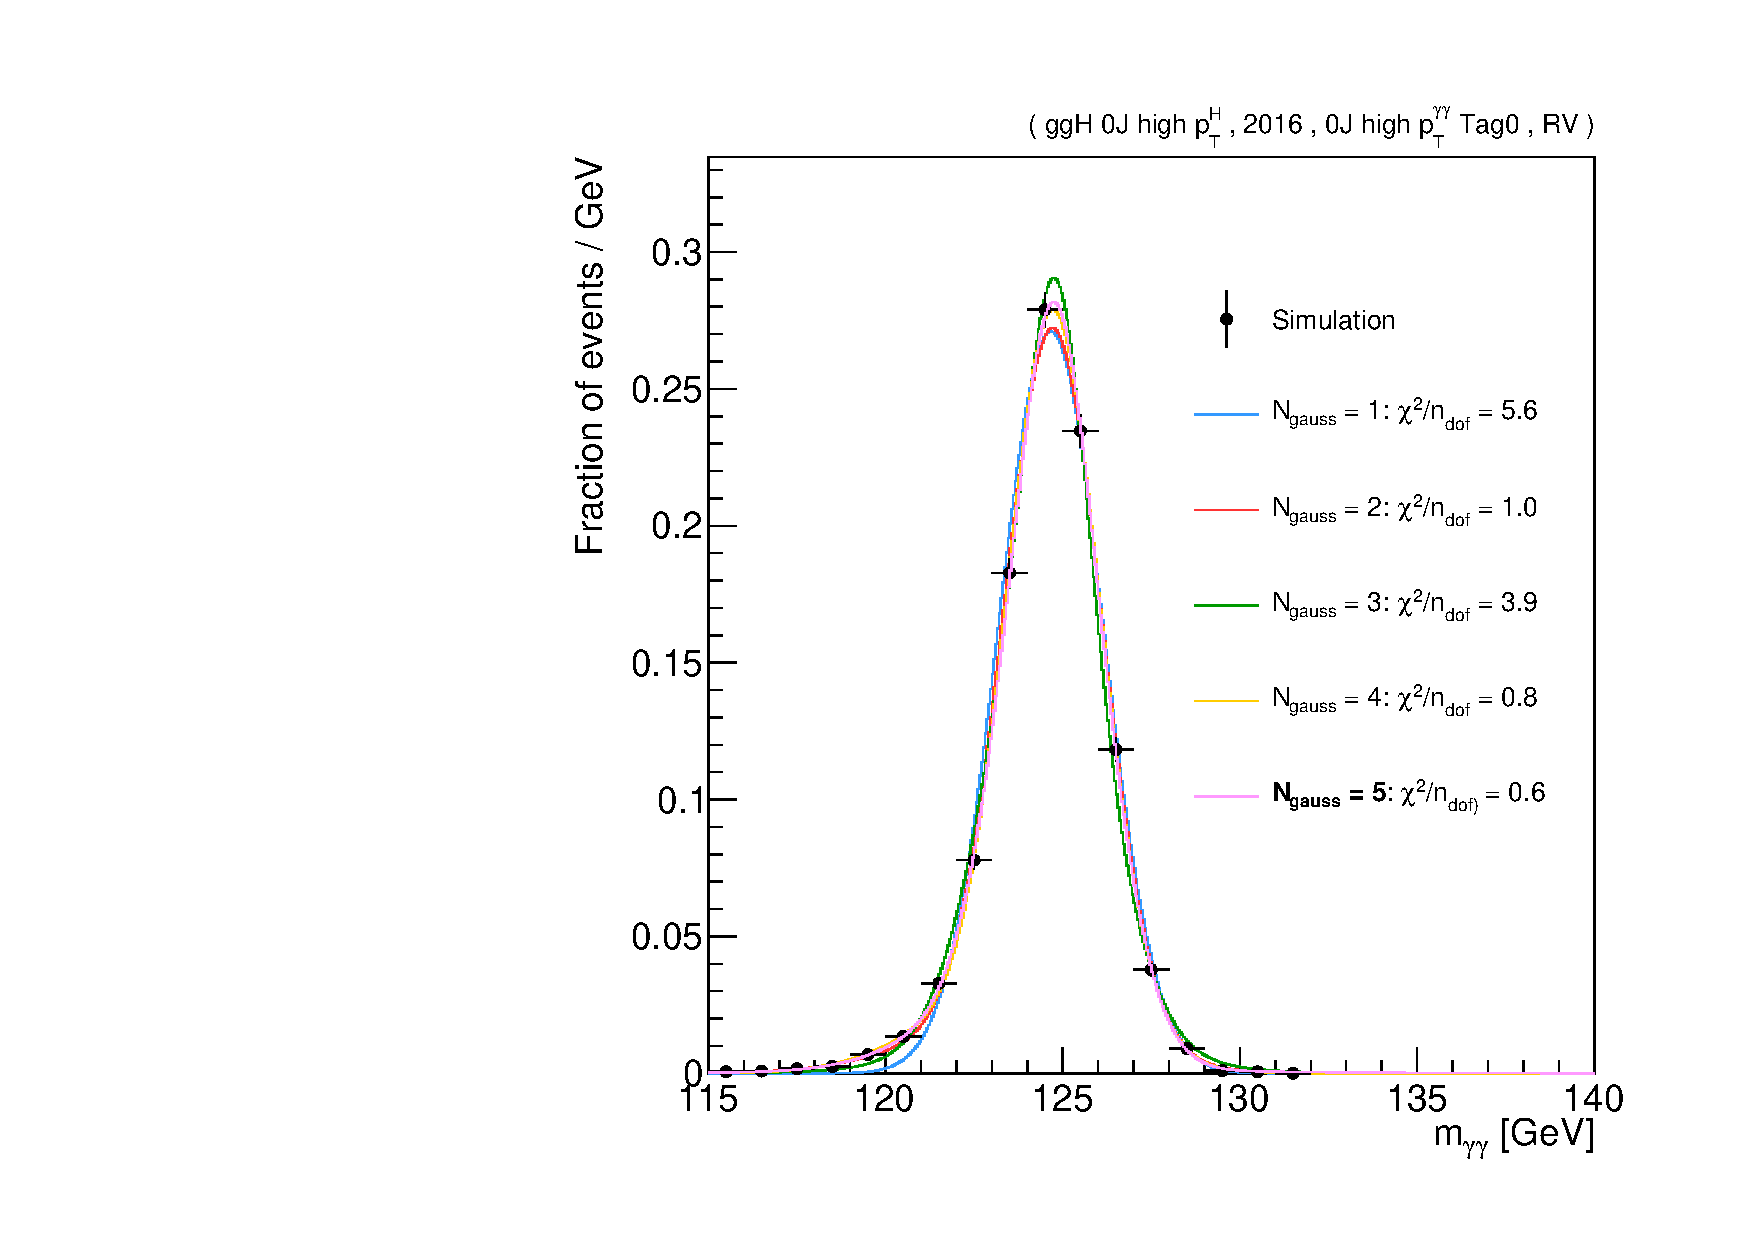
\includegraphics[width=.49\textwidth]{Figures/hgg_stats/fTest_RECO_0J_PTH_GT10_Tag0_GG2H_0J_PTH_GT10_RV.pdf}
  \hfill
  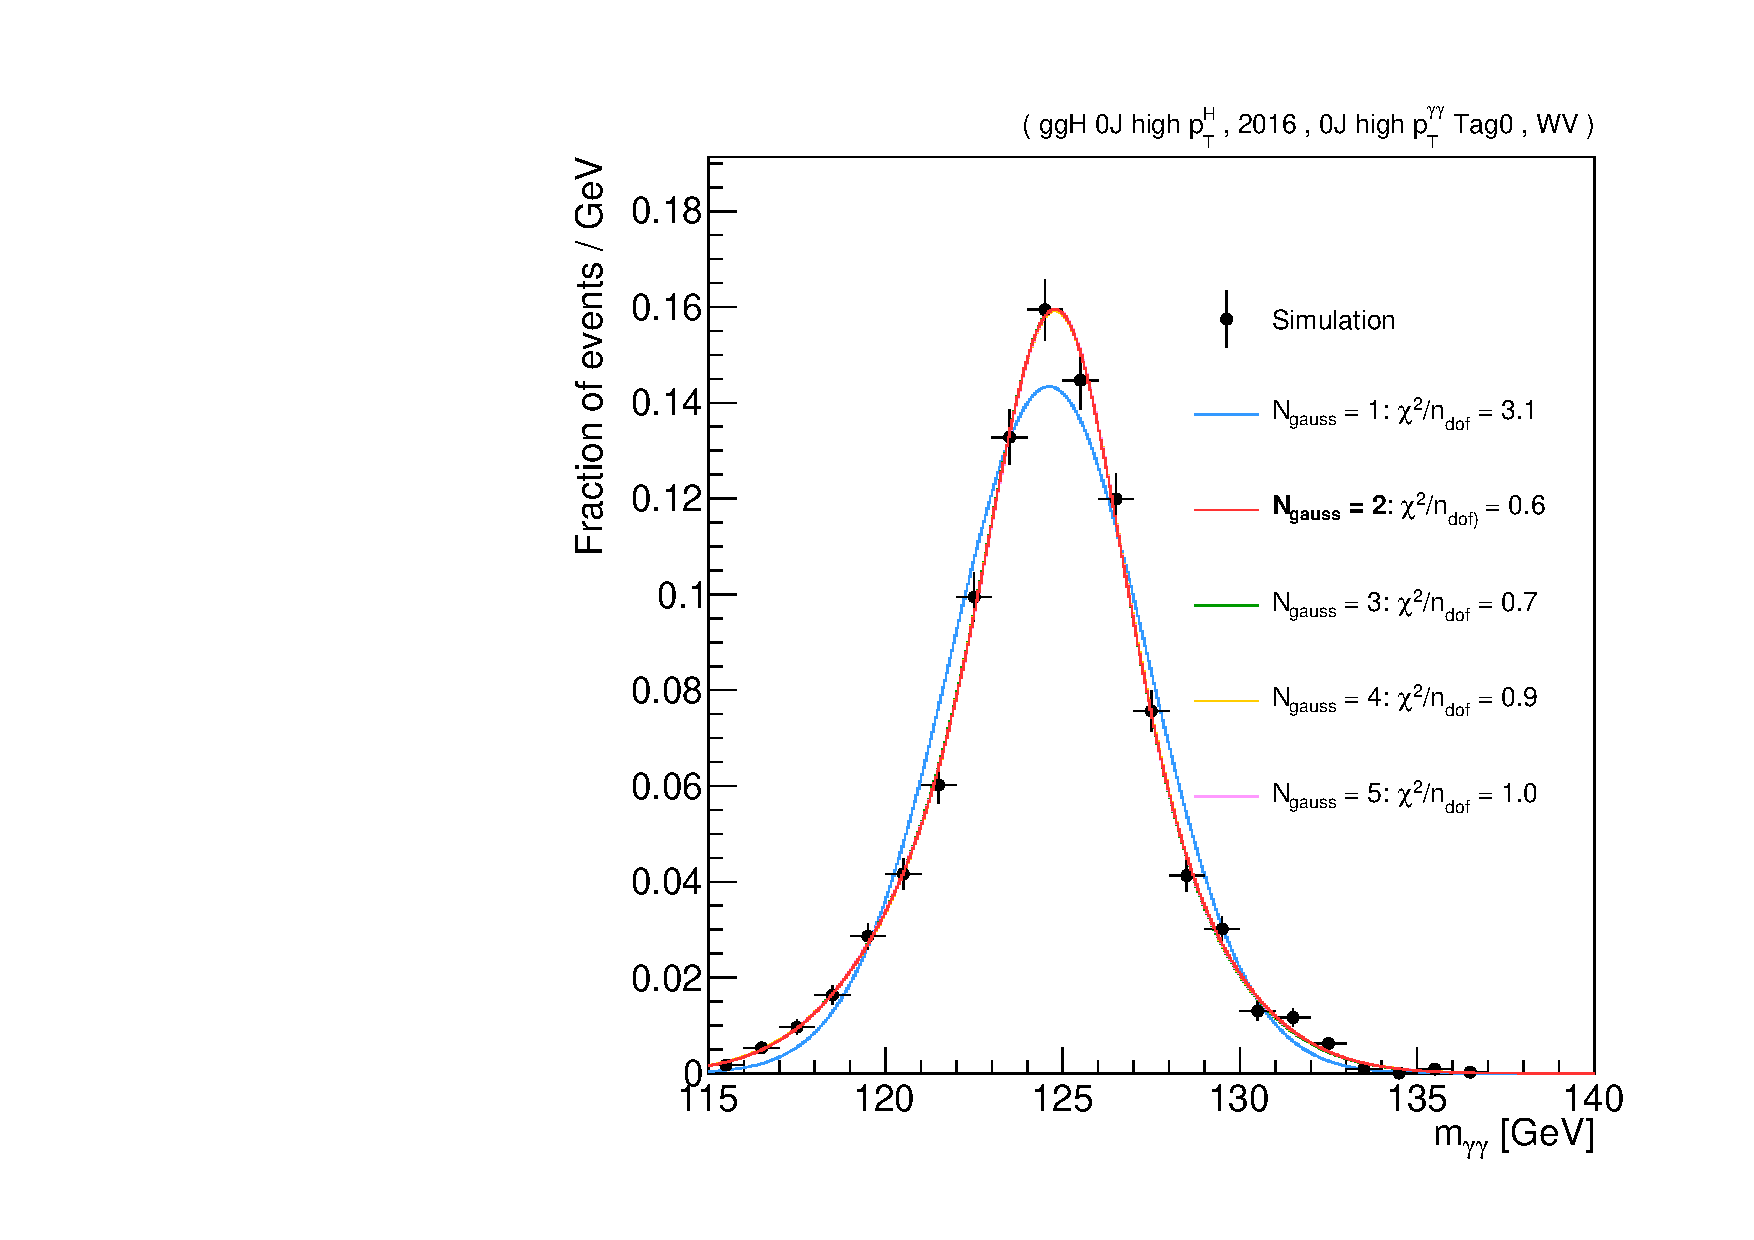
\includegraphics[width=.49\textwidth]{Figures/hgg_stats/fTest_RECO_0J_PTH_GT10_Tag0_GG2H_0J_PTH_GT10_WV.pdf}
  \caption[Signal modelling: number of Gaussians]
  {
    Finding the optimal number of Gaussian functions to fit the signal peak for ggH 0J high \ptH events in the 0J high \ptgg Tag0 category, from 2016 simulation with $m_H$~=~125.0~GeV. Events in the RV and WV scenarios are shown in the left and right plots, respectively. Up to five Gaussian functions are trialed for each vertex scenario. The optimal choices are 5 Gaussians for the RV events and 2 Gaussians for the WV events.
  }
  \label{fig:sigmodels_ftest}
\end{figure}

\begin{figure}
  \centering
  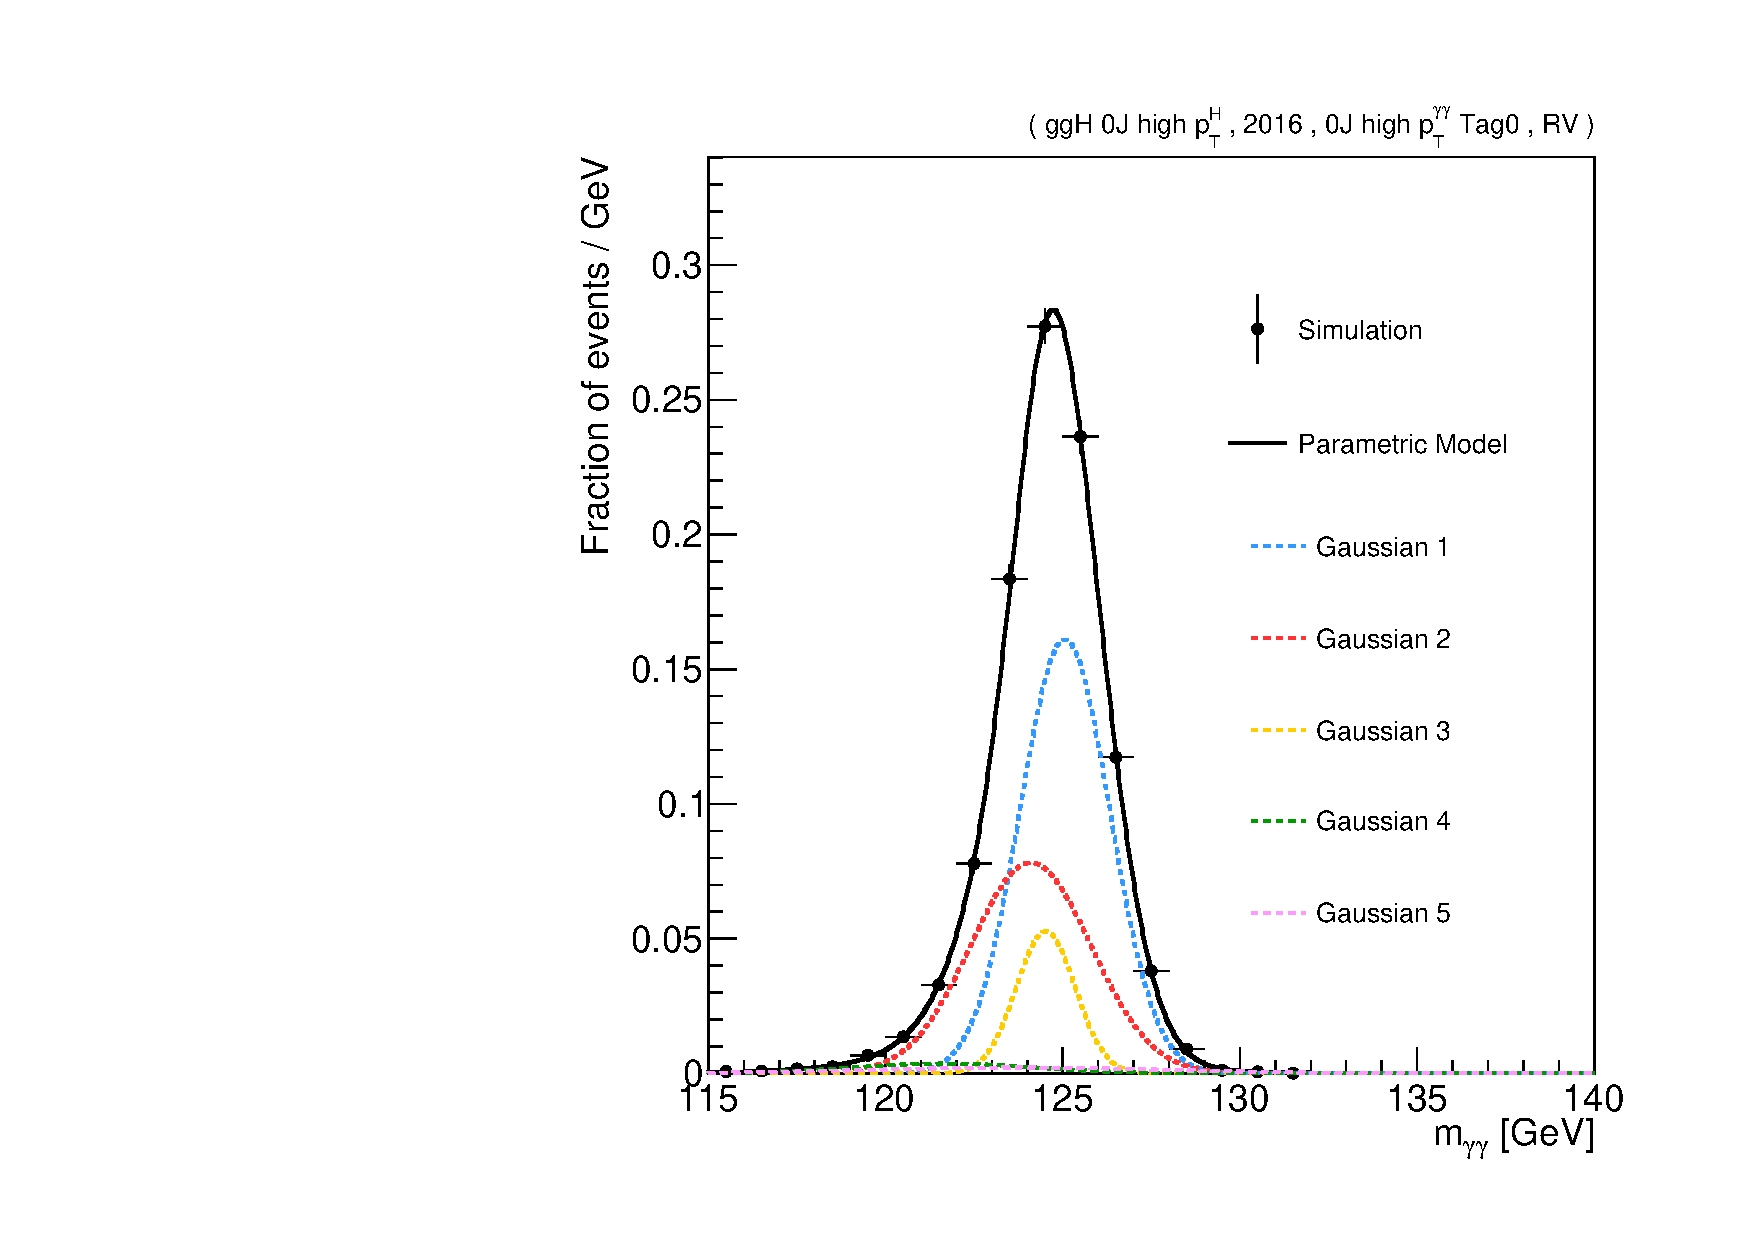
\includegraphics[width=.49\textwidth]{Figures/hgg_stats/RV_shape_pdf_components_GG2H_0J_PTH_GT10_RECO_0J_PTH_GT10_Tag0.pdf}
  \hfill
  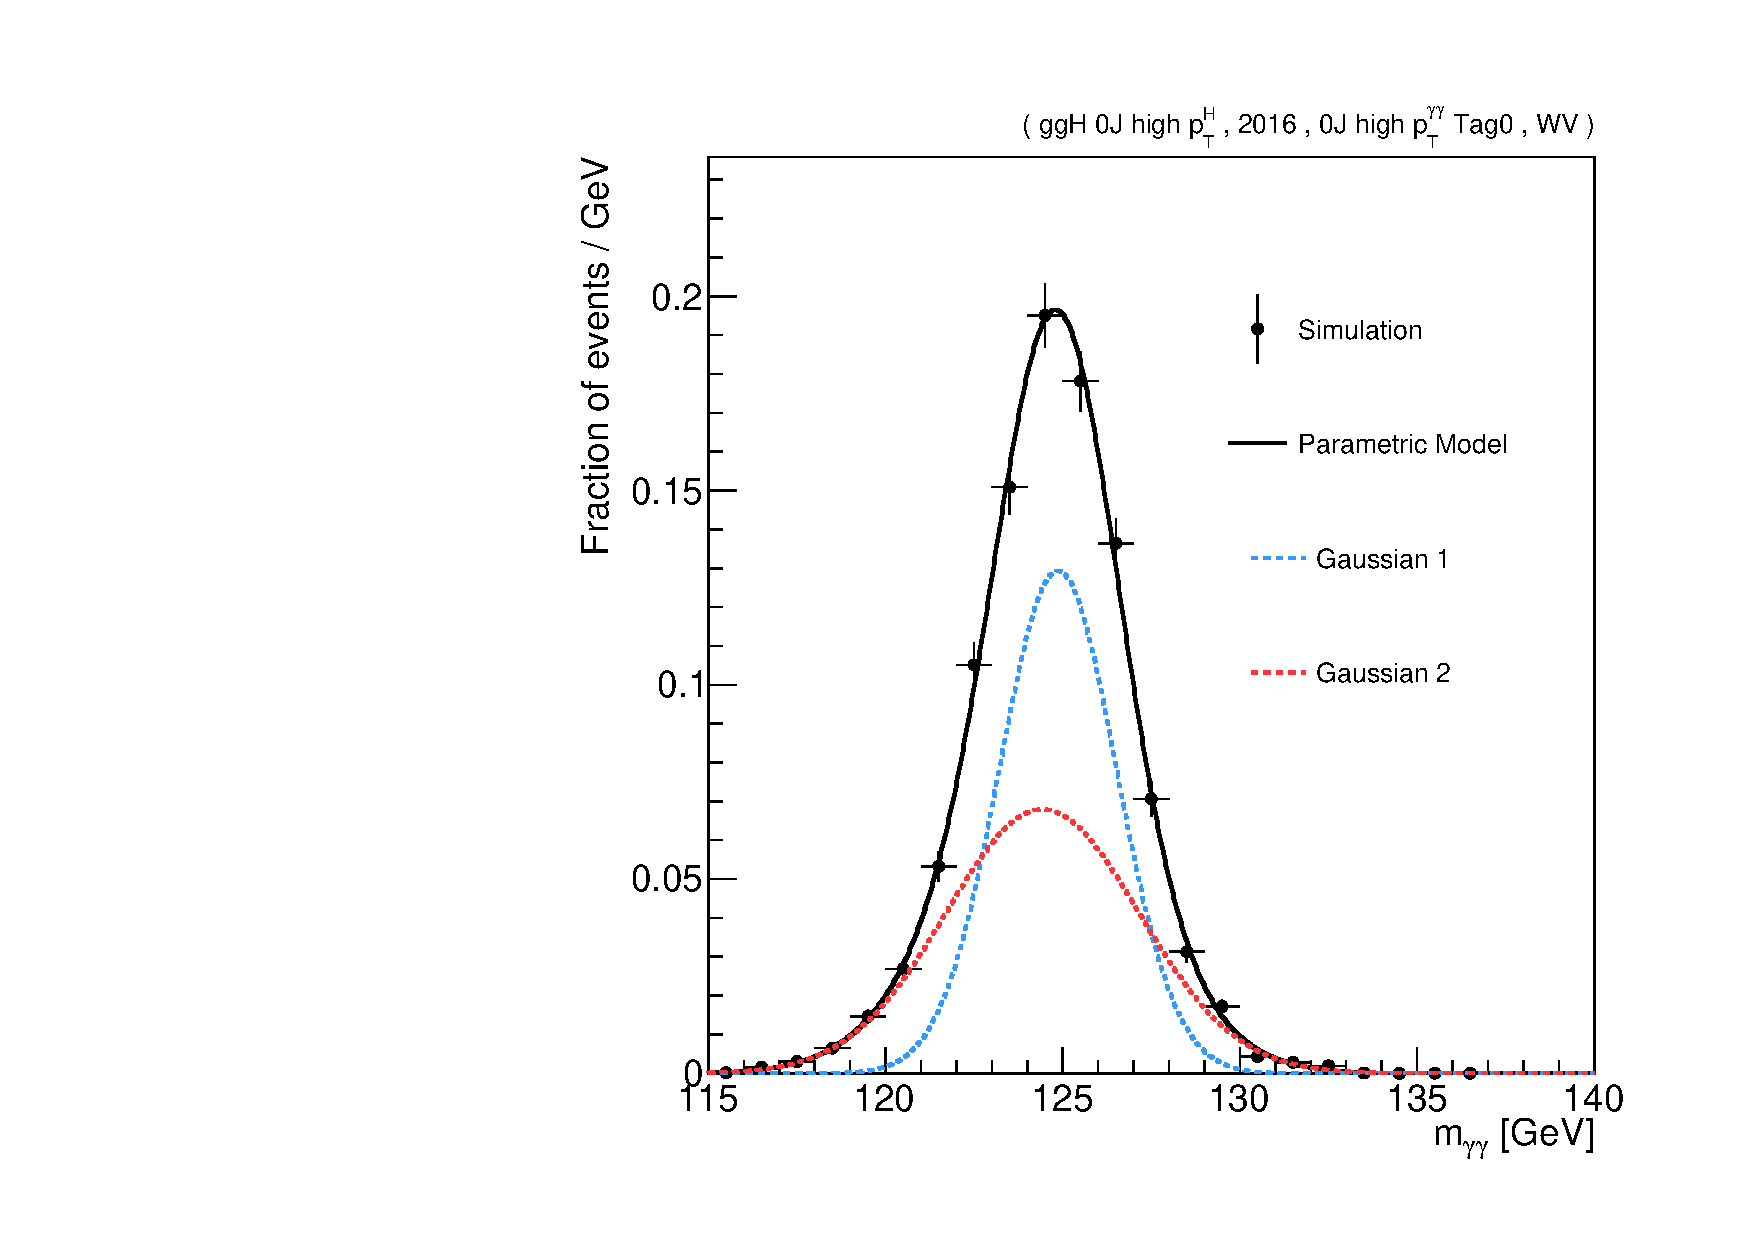
\includegraphics[width=.49\textwidth]{Figures/hgg_stats/WV_shape_pdf_components_GG2H_0J_PTH_GT10_RECO_0J_PTH_GT10_Tag0.pdf}
  \caption[Signal modelling: components]
  {
    The final signal model shapes (black lines) for ggH 0J high \ptH events in the 0J high \ptgg Tag0 category, from 2016 simulation with $m_H$~=~125.0~GeV (black points). Events in the RV and WV scenarios are shown in the left and right plots, respectively. In each case, the total shape is decomposed into the individual Gaussian functions, shown by the coloured lines.
  }
  \label{fig:signal_fitting}
\end{figure}

For a number of ($i$,$k$,$V$) combinations, particularly those corresponding to the far off-diagonal elements in Figure \ref{fig:purity_matrix}, there is an insufficient number of simulated events to accurately model the signal shape. In this case, the shape is replaced by that of the diagonal process, or in other words the STXS bin with the highest yield in analysis category, $k$. This replacement is motivated by the fact that events in the same region of experimental phase space i.e subject to the same selection criteria, tend to have similar values of the diphoton mass resolution.

The signal models are normalised according to equation \ref{eq:signal_yield}. The SM predictions of the cross sections and the \Hgg branching fraction, evaluated at $m_H=125.38$~GeV, are taken from Ref.~\cite{deFlorian:2016spz}, and the fractional breakdowns into the respective STXS bins are calculated directly from the MC samples (see Tables~\ref{tab:ggH_definitions}--\ref{tab:top_definitions}). As mentioned above, the efficiency times acceptance terms, $\epsilon^{i,\gamma\gamma}_{k}$, are derived separately for each year. The values are calculated directly from SM MC simulation with $m_H$~=125.0~GeV, as the fraction of the total yield of STXS bin, $i$, that lands in analysis category, $k$. Again, this approach works under the fact that the variation in $\epsilon^{i,\gamma\gamma}_{k}$ is negligible in going from $m_H=125.0$~GeV to 125.38~GeV, and is well below the yield systematic uncertainties introduced in section \ref{sec:systematics_experimental}. This was explicitly checked using dedicated signal samples at $m_H$~=~120 and 130~GeV, and interpolating between mass points to obtain the efficiency times acceptance values at $m_H$~=~125.38~GeV. The inclusive efficiency times acceptance, defined as the fraction of the total signal yield landing in any category, was found to vary by less than 0.1\%. The $\epsilon^{i,\gamma\gamma}_{k}$ are shown separately for each year in Appendix~\ref{app:eff_acc}.

At this point it is worth reminding the reader of a particular property of STXS measurements: the experimental acceptance of events within a given STXS bin are assumed to take their SM values (as the $\epsilon^{i,\gamma\gamma}_{k}$ terms are extracted with SM simulation). In the presence of BSM physics, the event kinematics can be modified which in turn affects experimental acceptance. This assumption, which is explicitly discussed in the context of EFT in section~\ref{sec:eft_acceptance_corrections}, should be treated carefully when performing BSM interpretations of STXS measurements. 

% \begin{figure}[hptb]
%   \centering
%   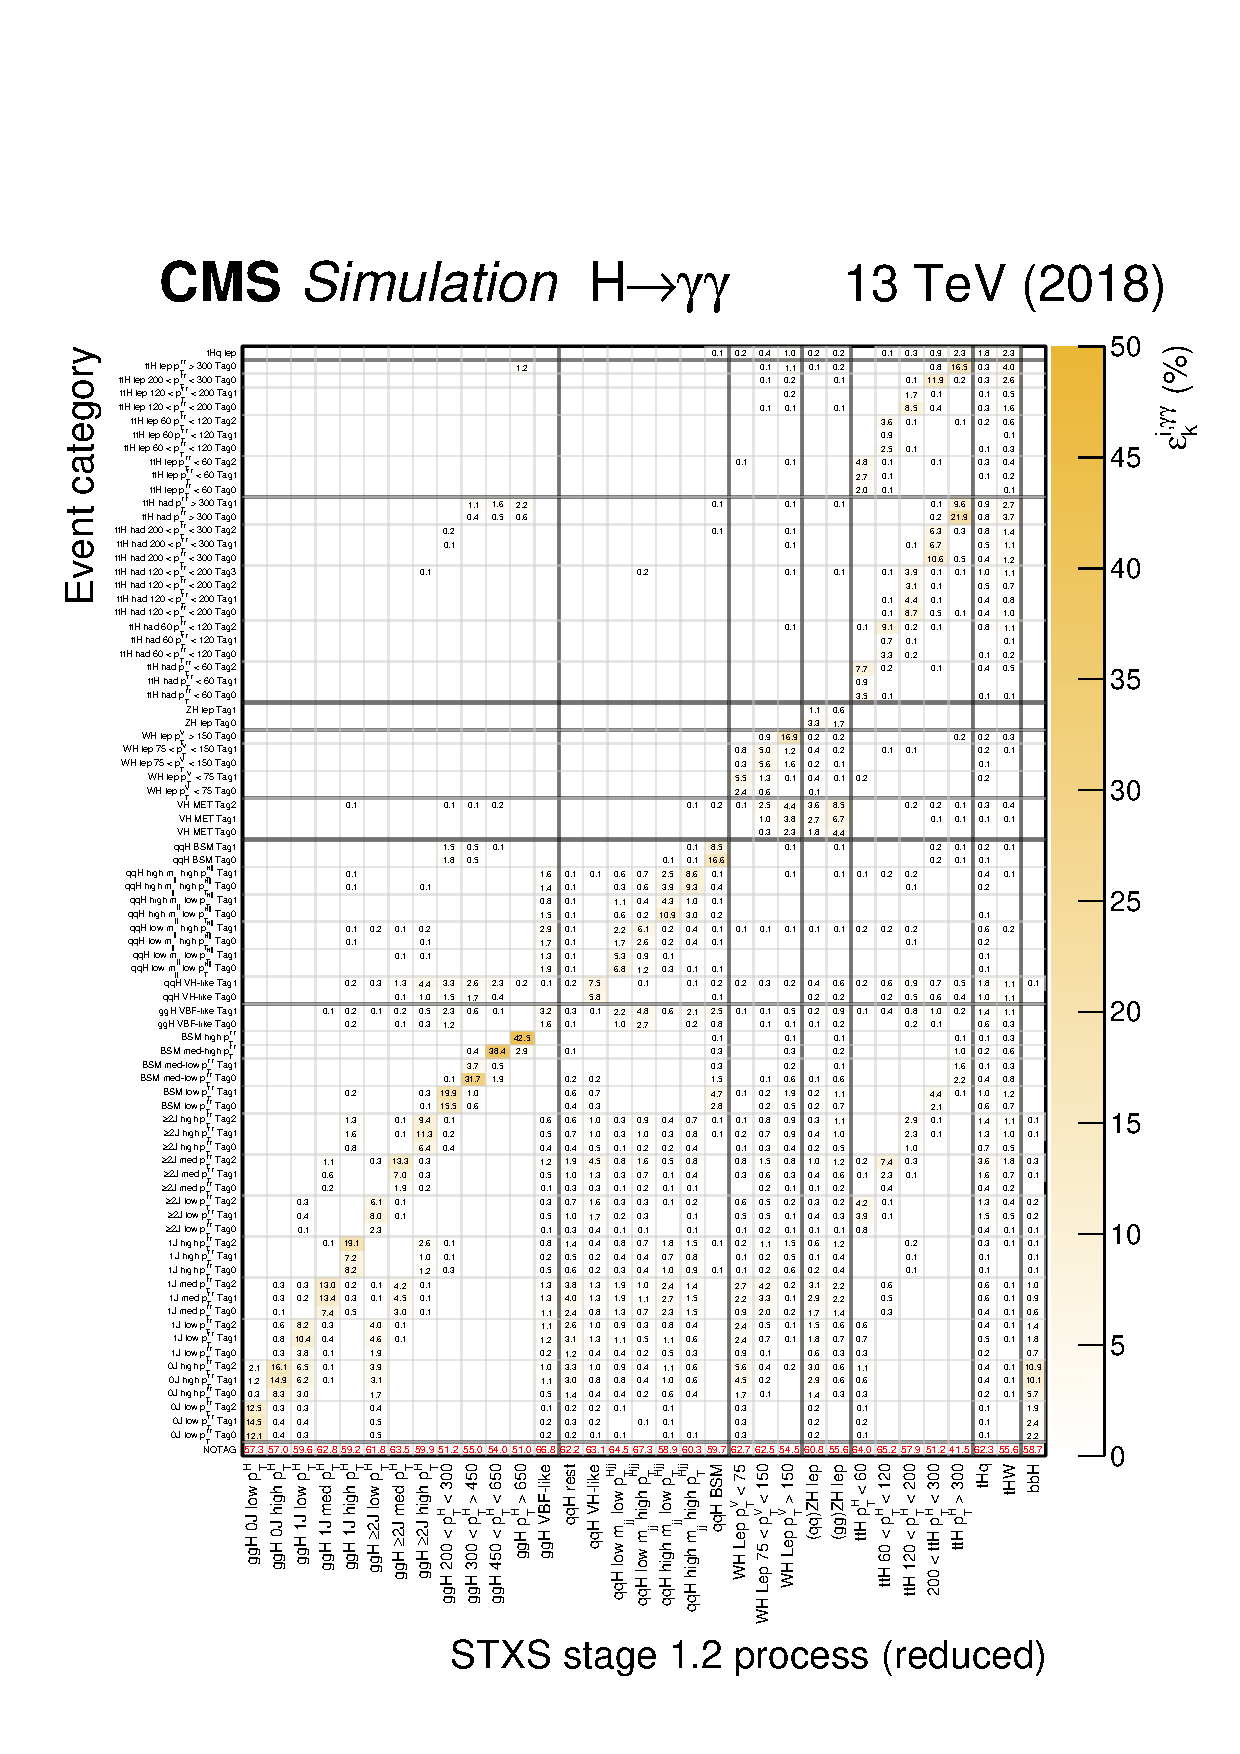
\includegraphics[width=1\textwidth]{Figures/hgg_stats/migrationMatrix_2018_thesis.pdf}
%   \caption[Efficiency times acceptance matrix from 2018 simulation]
%   {
%     A matrix showing the $\epsilon^{i,\gamma\gamma}_{k}$ terms for a reduced set of STXS bins, derived from 2018 simulation with $m_H$~=~125.0~GeV. The numbers corresponds to the fraction of the total yield of STXS bin, $i$, landing in analysis category, $k$, expressed as a percentage. Each column therefore sums to 100\%. Entries with values less than 0.05\% are not shown. The bottom row indicates the fraction of events which do not enter a single analysis category. The column labelled as qqH rest includes the contributions from the qqH 0J, qqH 1J, qqH $m_{jj}<60$~GeV and the qqH $120<m_{jj}<350$~GeV STXS bins.
%   }
%   \label{fig:ea_2018}
% \end{figure}

The per-category signal models are defined by summing the individual models of each STXS bin,
\begin{equation}
    \mathcal{S}_k = \sum_i \mathcal{S}^{i,\gamma\gamma}_k = \sum_i f_{RV} \cdot \mathcal{S}^{i,\gamma\gamma}_{k,RV} + (1-f_{RV}) \cdot\mathcal{S}^{i,\gamma\gamma}_{k,WV}.
\end{equation}
\noindent
Figure \ref{fig:sigmodels_category} shows the per-category signal models for the 0J high \ptH Tag0 and qqH VH-like Tag0 categories. The $\sigma_{\rm{eff}}$, defined as half of the smallest interval containing 68.3\% of the invariant mass distribution, is used to quantify the diphoton mass resolution. In the plots, the models are split into the contributions from each year, and the respective $\sigma_{\rm{eff}}$ values are displayed. In general, the detector performance, and therefore the diphoton mass resolution, worsen as a function of time due to radiation damage in the electromagnetic calorimeters. However, an extensive and thorough offline reconstruction program was developed specifically for the 2017 data, resulting in improved diphoton mass resolution and therefore smaller values of $\sigma_{\rm{eff}}$. Such offline reconstruction programs will be performed by the CMS collaboration for the 2016 and 2018 data in the future. 

\begin{figure}[hptb]
  \centering
  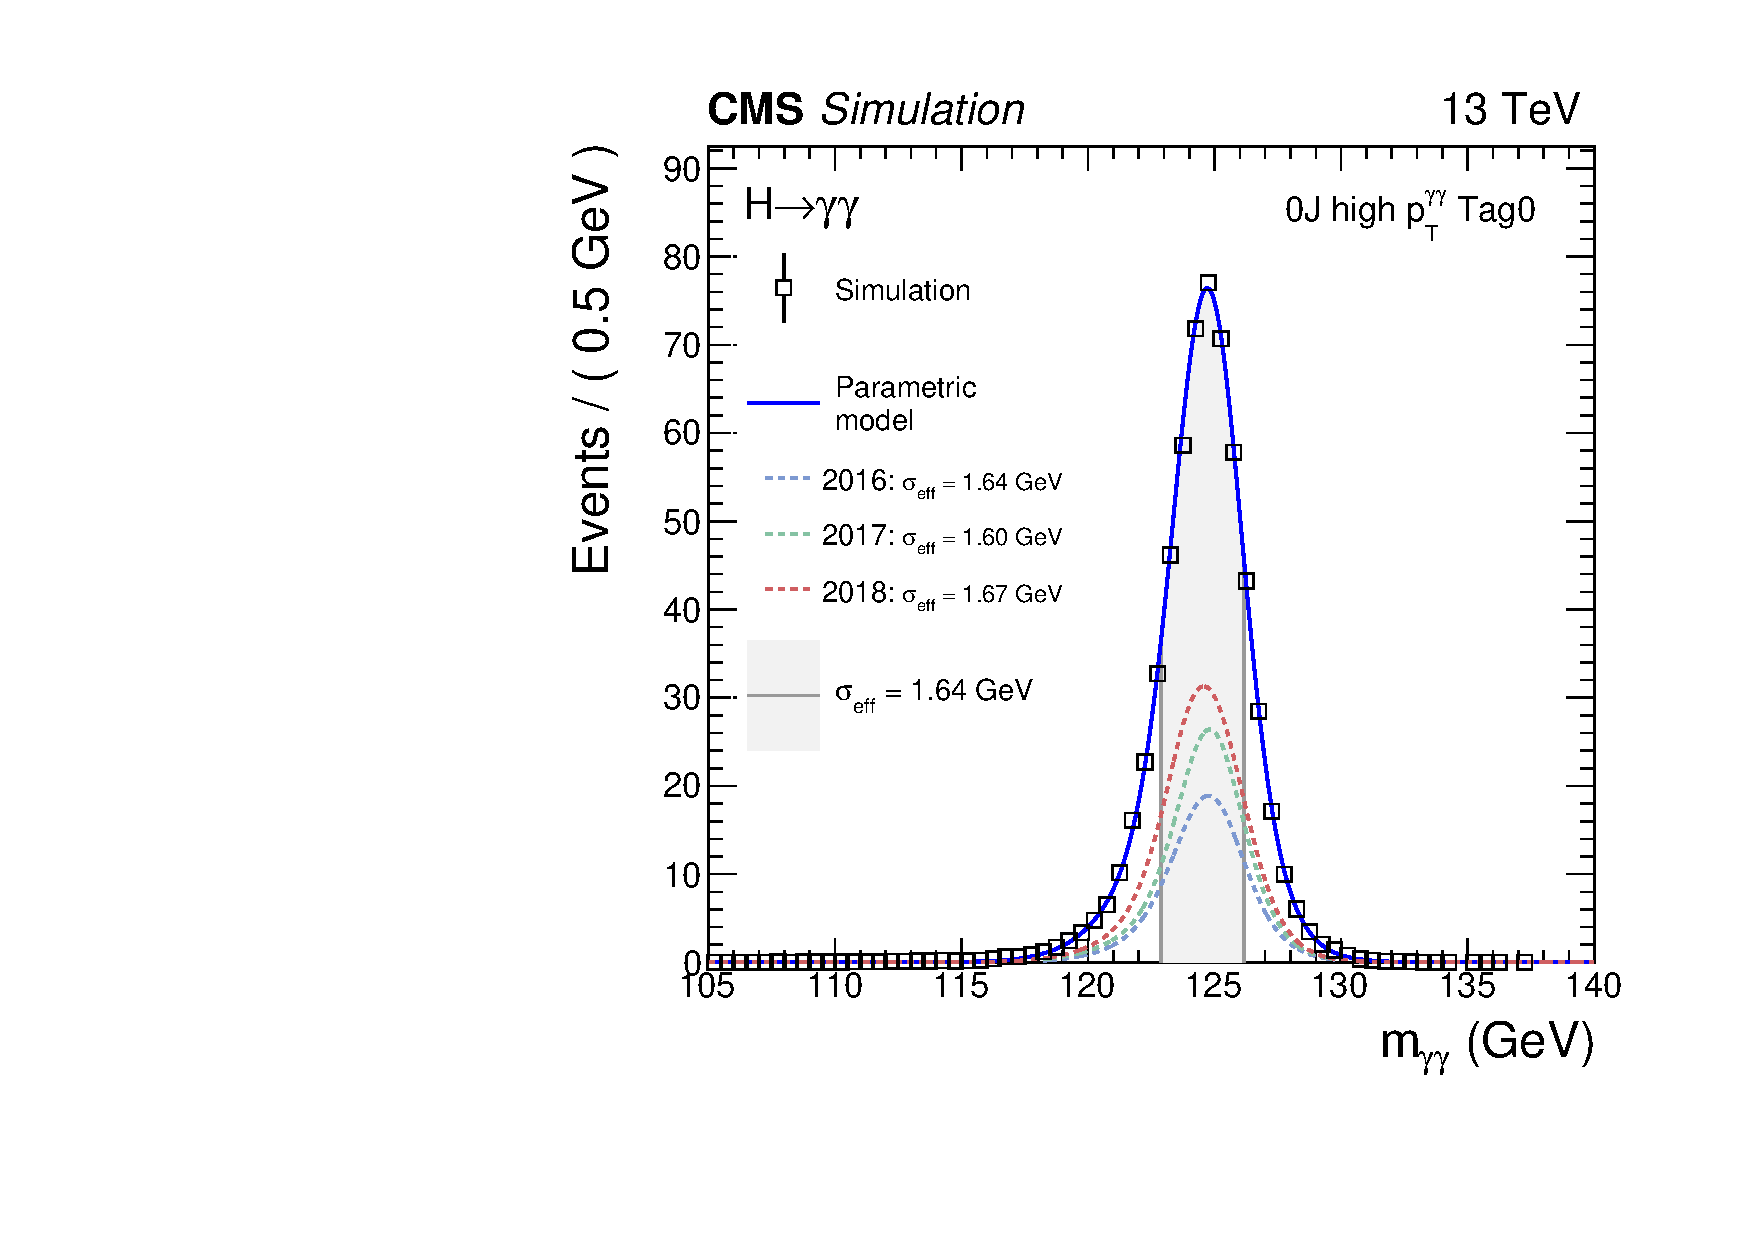
\includegraphics[width=.45\textwidth]{Figures/hgg_stats/smodel_RECO_0J_PTH_GT10_Tag0.pdf}
  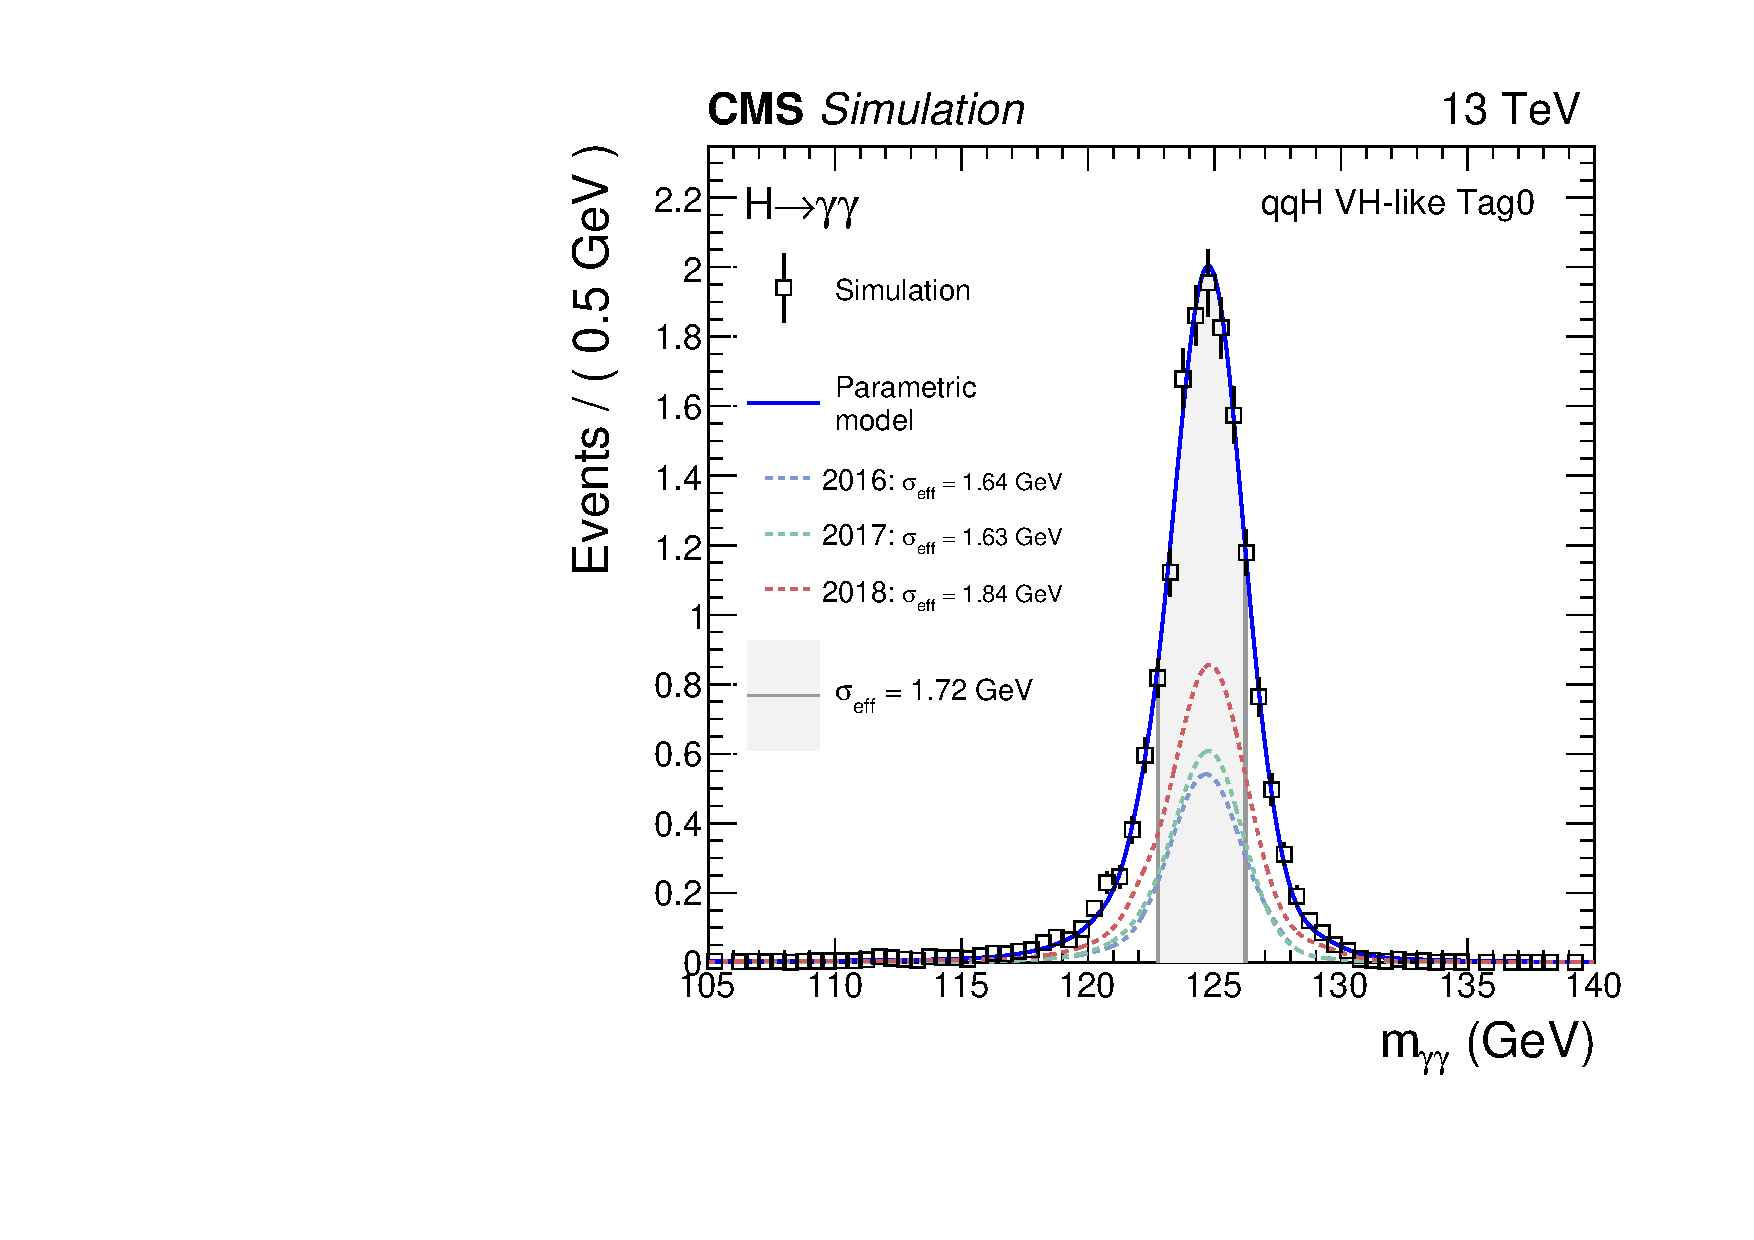
\includegraphics[width=.45\textwidth]{Figures/hgg_stats/smodel_RECO_VBFTOPO_VHHAD_Tag0.pdf}
  \caption[Signal models for the 0J high \ptgg Tag0 and qqH VH-like Tag0 categories]
  {
    Per-category signal models for the 0J high \ptH Tag0 (left) and qqH VH-like Tag0 (right) categories, shown for $m_H$~=~125.0~GeV. The model is shown for each year of simulated data (dashed lines) and for the sum of all years (solid line), normalised to the expected signal yield in each category. The open squares correspond to the simulated signal events. Also shown is the $\sigma_{\rm{eff}}$ in the grey shaded area. 
  }
  \label{fig:sigmodels_category}
\end{figure}

Going further, we can plot the sum of all per-category models to show the total signal model, $\mathcal{S}$. In Figure \ref{fig:sigmodels_weighted}, each per-category model is weighted in the sum according to the $F_{68} = S_{68}/(S_{68}+B_{68})$ values displayed in Tables \ref{tab:ggH_category_yields}--\ref{tab:top_category_yields}, such that the total signal yield remains constant. The explicit form of the weighted sum is shown in Equation \ref{eq:sigmodel_wsum}, where the index, $l$, runs over all analysis categories,

\begin{equation}\label{eq:sigmodel_wsum}
    \mathcal{S}^' = \sum_k w_k\,\mathcal{S}_k; \qquad w_k = (F^k_{68}) \times \frac{\sum_l S^l_{68}}{\sum_l F^l_{68} S^l_{68}}.
\end{equation}

\begin{figure}[hbtp]
  \centering
  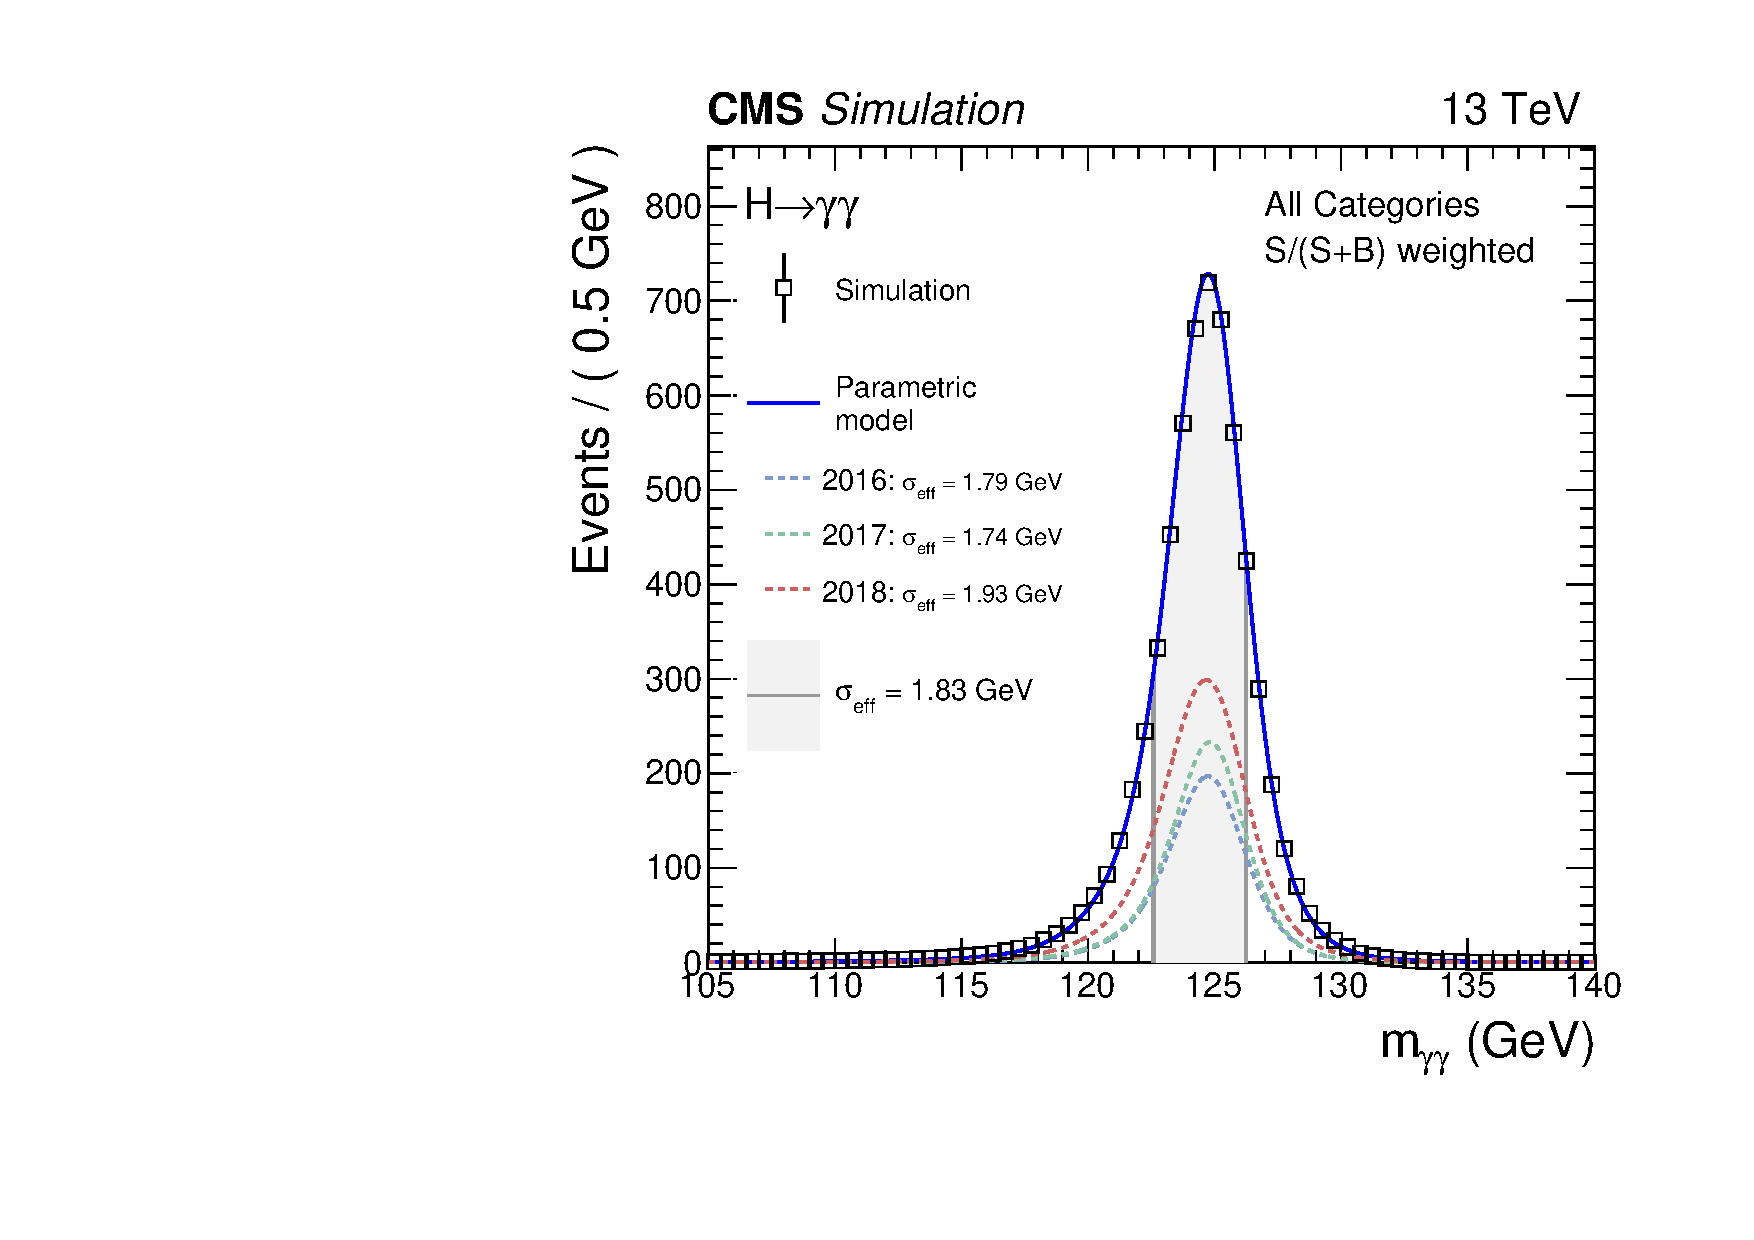
\includegraphics[width=.45\textwidth]{Figures/hgg_stats/smodel_all_weight.pdf}
  \caption[Weighted sum of all signal models]
  {
    The total signal model is shown for $m_H~=~125.0$~GeV, defined as the weighted sum of all per-category signal models. In the sum each category is weighted according to $F_{68}=S_{68}/(S_{68}+B_{68})$, such that the total signal yield remains constant.
  }
  \label{fig:sigmodels_weighted}
\end{figure}

\newpage
\section{Background modelling}\label{sec:bkg_modeling}
Events entering the analysis categories that do not originate from Higgs boson production form a smoothly falling \mgg distribution, on top of which the signal peak resides. To derive the $B_{k,X}$ terms of equation \ref{eq:category_likelihood}, an analytic model is constructed in each analysis category to describe the distribution of background events. These models are extracted directly from data.

The underlying shape of the background distribution is not \textit{a priori} known, and therefore a number of functional forms must be considered. Ultimately, this analysis amounts to measuring a small Higgs boson signal sitting on top of a larger background. As a result, relatively small changes in the background model shape and thus the estimated background contribution under the signal peak, may incur a large variation in the measured signal parameters of interest. The uncertainty in the choice of background function must therefore be accounted for.

\subsection{The effect of nuisance parameters on the likelihood}\label{sec:effect_of_nuisance}
Before introducing the background modelling procedure in detail, it is worth taking time to understand the effect of nuisance parameters on the likelihood. When minimising the quantity $-2\ln{L}$, the nuisance parameters representing systematic uncertainties are profiled: their value is free to vary during the minimisation, in accordance with the specified constraint $\mathcal{C}$, but their final value is not of interest. The increased freedom in the fit means that for a given point in parameter space, $\vec{\alpha}$, a configuration of the nuisance parameters can be found, $\vec{\theta}_{\vec{\alpha}}$, which increases the likelihood, $L|_{\vec{\alpha}}$, or equivalently decreases the value of $-2\ln{L}|_{\vec{\alpha}}$. This manifests as a widening of the $q(\vec{\alpha})$ curve, and therefore an increase of the uncertainty in the fitted parameters of interest.

The contribution to the total uncertainty from an individual nuisance parameter, $\theta$, is realised by fixing the nuisance parameter to it's best-fit value, $\hat{\theta}$, in the fit. The width of the resulting $q(\vec{\alpha})$ curve represents the total uncertainty without the effect of $\theta$, and therefore will be narrower than curve in which $\theta$ is profiled. Ignoring correlation effects between nuisance parameters, we can define the contribution to the uncertainty from $\theta$ as the quadrature-difference in the curve widths. In this analysis, we use this technique to evaluate the \textit{impact} of each uncertainty source on the parameters of interest. In addition, by fixing groups of nuisance parameters to their best-fit values, it is possible to decompose the total uncertainty into contributions from theoretical sources ($\vec{\theta}^{\,\rm{th}}_{s}$, $\vec{\theta}^{\,\epsilon,{\rm{th}}}_{s}$), experimental sources ($\vec{\theta}^{\,\epsilon,{\rm{exp}}}_{s}$, $\vec{\theta}^{\,\rm{shape}}_{s}$, $\vec{\theta}^{\,\rm{lumi}}_{s}$), and the statistical component\footnote{Here, the background model nuisance parameters, $\vec{\theta}^{\,\rm{shape}}_{b}$, $\vec{\theta}^{\,\rm{discrete}}_{b}$, are grouped with the statistical uncertainty.}. 

Figure \ref{fig:nuisance_illustration} illustrates a different approach to the same conclusion. The blue curve represents a fit in which the nuisance parameter in question, $\theta$, is fixed to it's best-fit value. By fixing $\theta$ to different values, it is possible to build up a series of likelihood curves, shown by the dashed red lines, with minima shifted from the unconditional best-fit point. The minimum envelope of these likelihood curves, shown by the dashed green line, can be used to approximate the contribution to the uncertainty from $\theta$. In the limit of infinitesimally small steps in $\theta$, the envelope converges to the fully profiled likelihood curve (black line).

\begin{figure}[hptb]
  \centering
  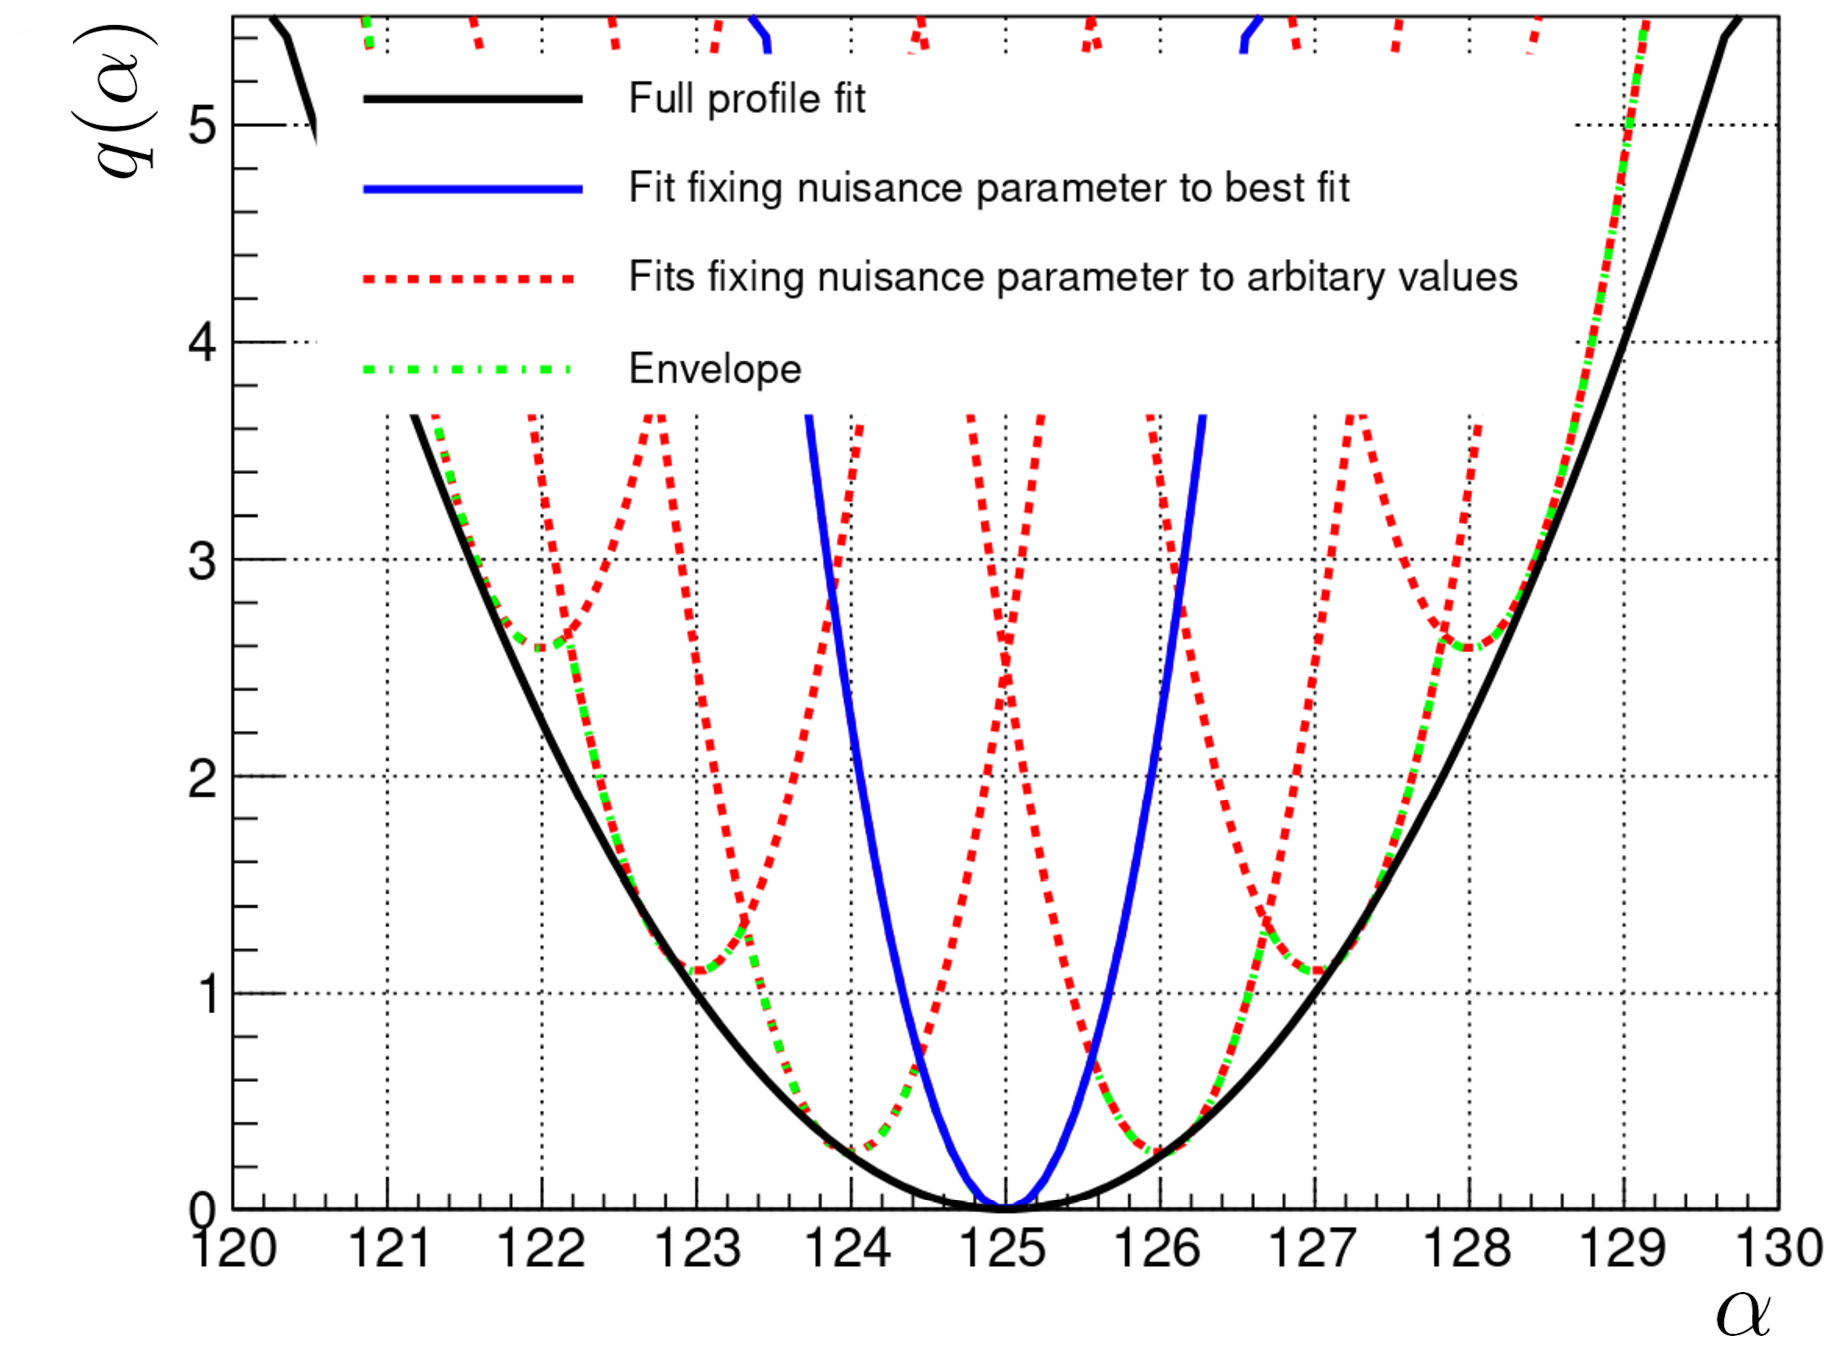
\includegraphics[width=.6\textwidth]{Figures/hgg_stats/nuisance_illustration.pdf}
  \caption[Constructing the envelope]
  {
    An illustration of constructing the envelope. The blue $q(\vec{\alpha})$ curve corresponds to a fit in which a nuisance parameter is fixed to its best-fit value. The red dashed lines show the curves obtained from fits where the nuisance parameter is fixed to different values. The minimum envelope of these curves is shown by the dashed green line. By sampling a sufficient number of difference nuisance parameter values, the envelope approximately models the fully profiled likelihood curve (black line). Figure taken from Ref.~\cite{Dauncey:2014xga}.
  }
  \label{fig:nuisance_illustration}
\end{figure}

\subsection{Discrete profiling method}
The example described above was introduced in the context of a continuous nuisance parameter. This same approach of building the envelope can be extended to the discrete case, where the nuisance parameter is limited to discrete values, albeit provided there is sufficient freedom in the allowed values to provide good coverage of the uncertainty.

In this analysis, the so-called \textit{discrete profiling method} is applied to model the uncertainty in the choice of background function~\cite{Dauncey:2014xga}. A number of candidate functions are considered to fit the background in each category, and a discrete nuisance parameter is introduced to label the choice of function. In theory, the complete set of all analytic functions should be considered to obtain the exact uncertainty; in practice it is sufficient to consider a subset of functions which provide a reasonable fit to data. This keeps the computing time required for the full minimisation to a tolerable level. By allowing the value of the discrete nuisance, and thus the functional form of the background to vary, an envelope of likelihoods is constructed (as in Figure \ref{fig:nuisance_illustration}) which successfully approximates the uncertainty in the choice of background function.

\begin{table}[htb]
    \caption[Function families considered in the discrete profiling method]{Different function families considered in the discrete profiling method. Each function is shown for order, $N$.}
    \label{tab:discrete_functions}
    \vspace{.5cm}
    \centering
    \footnotesize
    \renewcommand{\arraystretch}{1}
    \begin{tabular}{m{0.35\textwidth}|p{0.55\textwidth}}
       \begin{tabular}{l} ~\\~\\ Sum of exponentials\end{tabular} & 
       \begin{equation*}
           f_N(x) = \sum^N_{i=0} p_{2i}\,{\rm{exp}}\big( p_{2i+1}x\big)
       \end{equation*} \\ \hline
       \begin{tabular}{l} ~\\~\\ Sum of power law functions\end{tabular} & 
       \begin{equation*}
           f_N(x) = \sum^N_{i=0} p_{2i}x^{-p_{2i+1}}
       \end{equation*} \\ \hline
       \begin{tabular}{l} ~\\~\\ Bernstein polynomials\end{tabular} & 
       \begin{equation*}
           f_N(x) = \sum^N_{i=0} p_i {N \choose i}x^i(1-x)^{N-i}
       \end{equation*} \\ \hline
       \begin{tabular}{l} ~\\~\\ Laurent series\end{tabular} &
       \begin{equation*}
           f_N(x) = \sum^N_{i=0} p_i x^{-4+g(i)}; \qquad g(i) = \sum^i_{j=0} (-1)^jj
       \end{equation*} \\      
    \end{tabular}
\end{table}

The different families of functions considered are listed in Table~\ref{tab:discrete_functions}. For each family, the form is shown for order, $N$, uniquely described by parameters: $p_0$, $p_1$, ..., $p_N$. The following procedure is used to determine the final set of candidate functions for a given analysis category, $\mathcal{F}^k$:
\begin{itemize}
    \item A background-only fit is performed to the \mgg distribution in data, using the lowest-order function in a given family. This is performed by minimising the value of $-2\ln{L}_b$, allowing the parameters of the function to vary, where the subscript $b$ has been added to indicate this is a background-only fit ($S=0$). 
    %A penalty term, $P$, is added to $-2\ln{L}_b$, equal to the number of parameters in the function. This prevents functions with arbitrarily high freedom being chosen. 
    The process is repeated, incrementally raising the order, until a minimum goodness-of-fit criteria is reached. All orders below are not considered in $\mathcal{F}^k$ as they do not fit the data well.
    
    % \item For all subsequent orders, an F-test is performed to decide if the improvement in fit quality warrants the increase in function complexity~\cite{10.2307/2340521}. Using the same procedure, the $-2\ln{L}_b+P$ value is determined for the next-highest order function in the family. Given a large enough sample size, the difference in $-2\ln{L}_b+P$ values for successive orders, $\Delta$, is distributed according to the $\chi^2$ distribution with $m$ degrees of freedom, where $m$ is the difference in the number of parameters between the two orders. A $p$-value is calculated as,
    \item For all subsequent orders, an F-test is performed to decide if the improvement in fit quality warrants the increase in function complexity~\cite{10.2307/2340521}. Using the same procedure, the $-2\ln{L}_b$ value is determined for the next-highest order function in the family. Given a large enough sample size, the difference in $-2\ln{L}_b$ values for successive orders, $\Delta$, is distributed according to the $\chi^2$ distribution with $m$ degrees of freedom, where $m$ is the difference in the number of parameters between the two orders. A $p$-value is calculated as,
    
    \begin{equation}
        p = {\rm{Prob}}\Big(\Delta<\,\Delta_{\rm{obs}}\,\Big|\,\chi^2(m)\Big),
    \end{equation}
    \noindent
    where $\Delta_{\rm{obs}}$ is the observed value in data. If the $p$-value is less than 0.05 then the improvement in fit quality is deemed worthwhile, and the higher-order function is added to $\mathcal{F}^k$. This step is repeated for successive orders until the calculated $p$-value is larger than 0.05. In this scenario, the higher-order function is deemed to be unnecessarily complex given the data and the procedure terminates.

    \item This process is repeated for each of the four families listed in Table \ref{tab:discrete_functions}, where each order passing the above selection procedure enters $\mathcal{F}^k$.
\end{itemize}

The set of candidate functions, $\mathcal{F}^k$, are shown for the ggH 1J high~\ptgg Tag0 and ggH BSM low \ptgg Tag0 analysis categories in Figure \ref{fig:bkgmodels_category}. The different functional forms provide a different background estimate when integrating under the signal peak. This sometimes large variation in the background estimate gives rise to an uncertainty in the fitted signal parameters of interest, originating from the lack of knowledge of the true background functional form.

\begin{figure}[hptb]
  \centering
  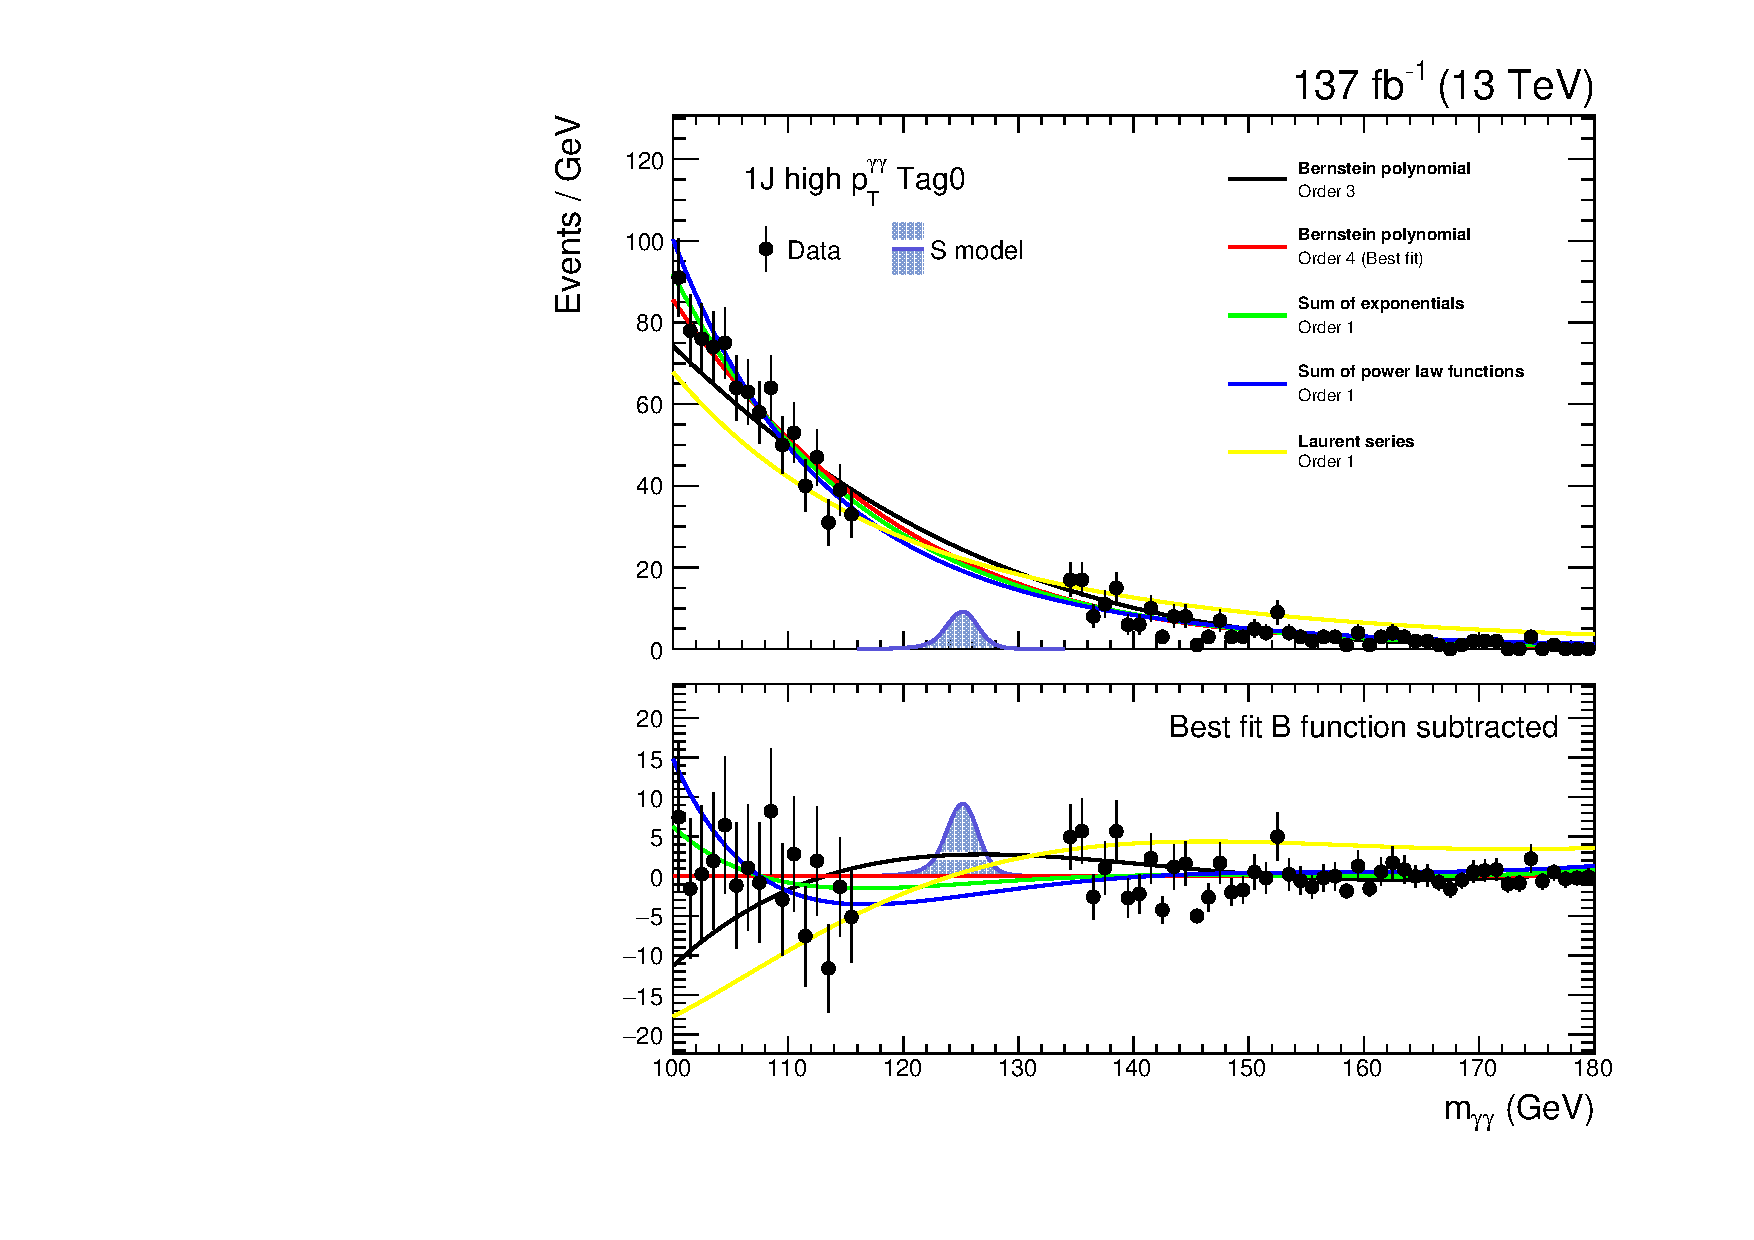
\includegraphics[width=.49\textwidth]{Figures/hgg_stats/bmodel_RECO_1J_PTH_120_200_Tag0.pdf}
  \hfill
  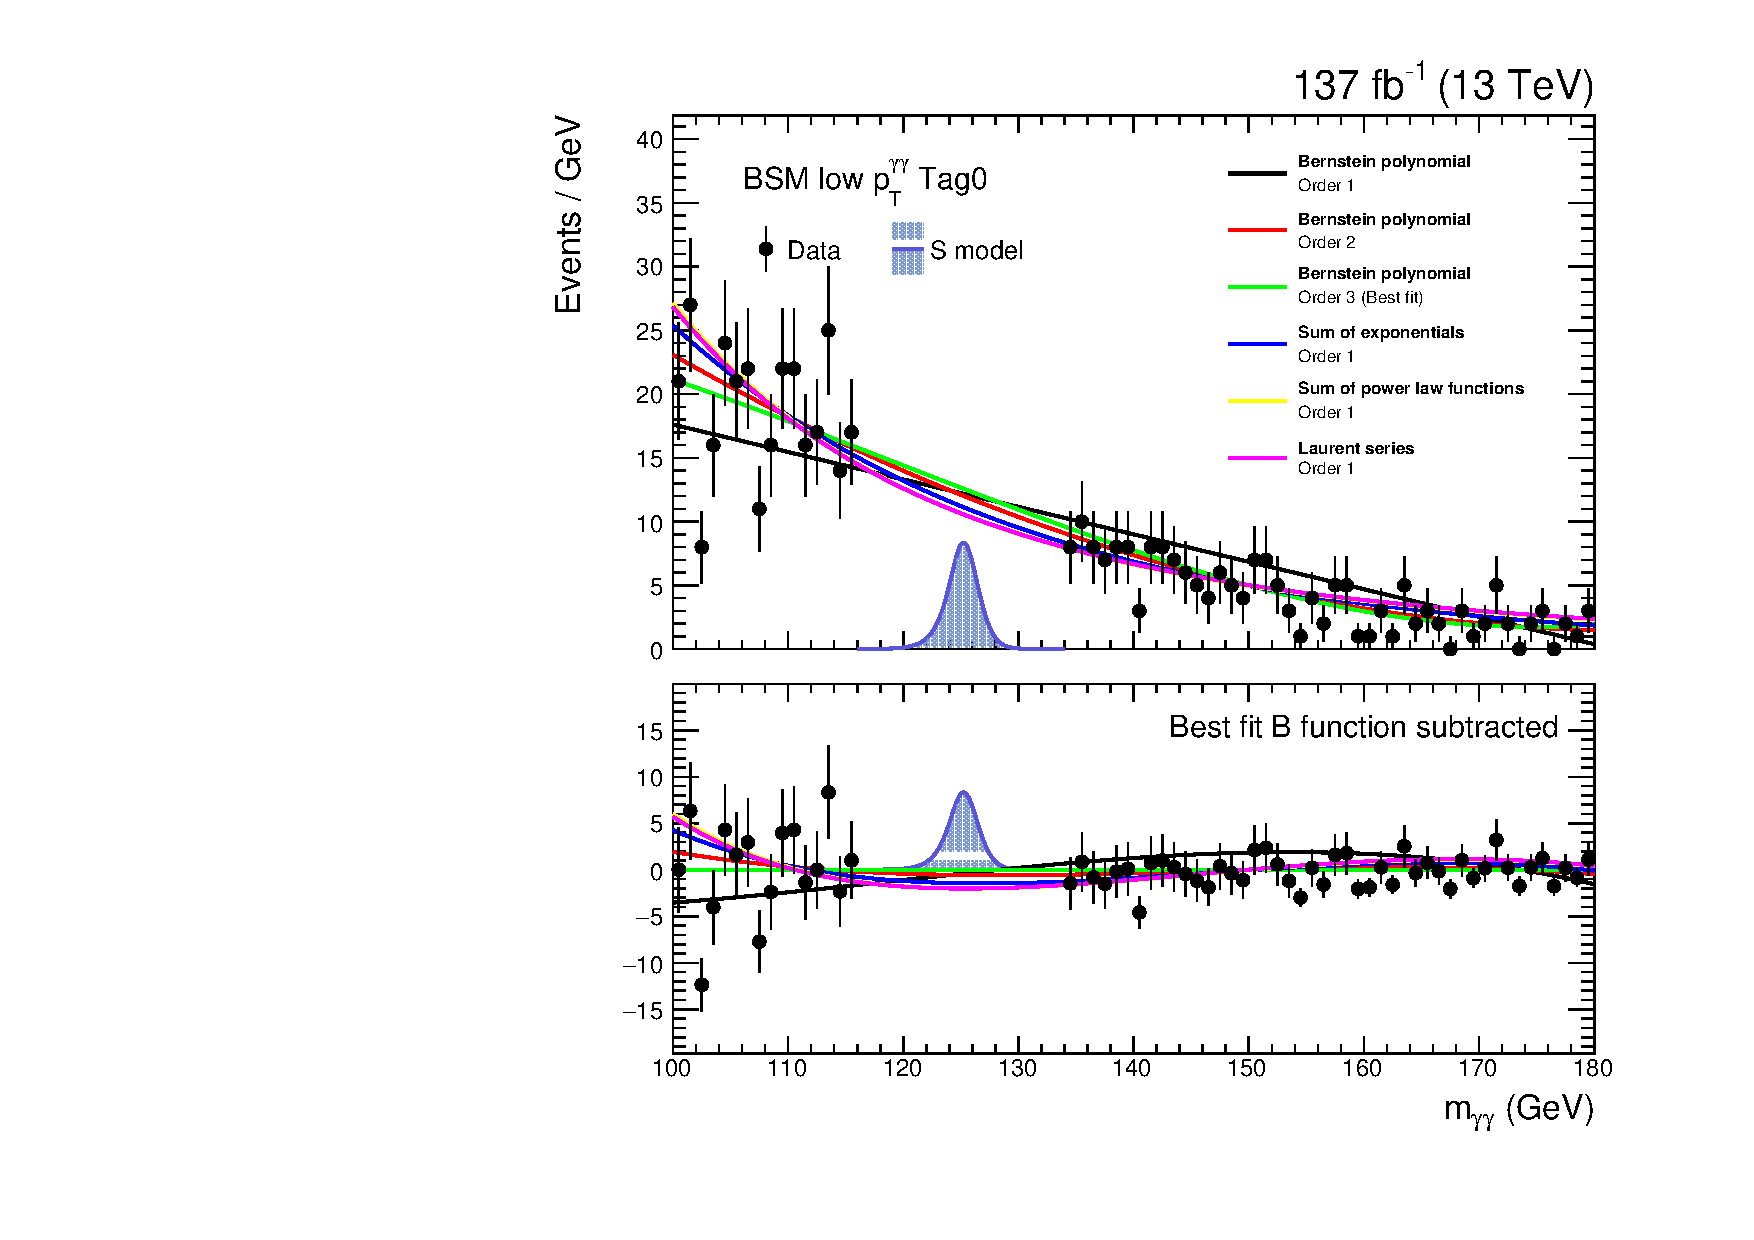
\includegraphics[width=.49\textwidth]{Figures/hgg_stats/bmodel_RECO_PTH_200_300_Tag0.pdf}
  \caption[Background models for the 1J high \ptgg Tag0 and qqH VH-like Tag0 categories]
  {
    The set of candidate functions, $\mathcal{F}^k$, considered in the final fit for the ggH 1J high~\ptgg Tag0 (left) and ggH BSM low \ptgg Tag0 (right) categories, shown by the coloured lines. Data events entering these analysis categories are shown by the black points, for diphoton invariant mass outside of the range $115<\mgg<135$~GeV. The corresponding signal models for the two categories are overlaid (filled blue histograms) to gain an idea of impact of the uncertainty in the choice of background function. The bottom panel in each plot shows the residuals after subtracting the best-fit background function in the background-only fit.
  }
  \label{fig:bkgmodels_category}
\end{figure}

In the final results extraction (see section \ref{sec:results_extraction}), both the discrete nuisance parameters describing the choice of background functions ($\vec{\theta}^{\,\rm{discrete}}_{b}$), and the parameters of the functions themselves ($\vec{\theta}^{\,\rm{shape}}_{b} \equiv p_0,...,p_N$) are free to vary. In accordance with the procedure described above, a penalty term is added to the value of $-2\ln{L}$ equal to the number of parameters in the chosen function, thus penalizing functions with high complexity. Further details concerning the discrete profiling method are provided in Ref.~\cite{Dauncey:2014xga}. This includes a series of tests to show the method provides good coverage of the uncertainty in the choice of background function and leads to unbiased estimates of the parameters of interest.

\section{Systematic uncertainties}\label{sec:systematics}
This section provides further detail on the sources of systematic uncertainty in the signal estimate, and how they are modelled using different types nuisance parameters. The uncertainties are divided into experimental sources and theoretical sources, described in sections \ref{sec:systematics_experimental} and \ref{sec:systematics_theoretical} respectively. For each source, the magnitude of the uncertainty's impact is calculated separately per year for each STXS bin in each analysis category.

\subsection{Uncertainty correlation scheme}\label{sec:correlation_scheme}
Before listing the various sources, it is important to introduce the concept of correlating nuisance parameters. As mentioned in section \ref{sec:sig_modelling}, the signal is modelled independently for the 2016, 2017, and 2018 data. This allows for a choice in the modelling of each uncertainty source. A correlated uncertainty means defining a single nuisance parameter in the final fit which affects the signal estimate in multiple years simultaneously. Note, this correlation may be defined for a pair of years, or can extend to a correlation across all three data-taking years. Alternatively, uncorrelated means defining a separate nuisance parameter for each year, such that the impacts on the signal estimates from each year are independent. 

Theoretical uncertainties are fully correlated across years. This somewhat trivial assignment is made since the underlying theoretical predictions are constant and do not depend on the data-taking conditions. In general, experimental sources are uncorrelated across years. This choice reflects the difference in data-taking conditions and data reconstructions for each year. Exceptions are the uncertainties in the luminosity estimate and the jet energy scale. For these, a partial correlation scheme is used i.e. a combination of uncorrelated and correlated nuisance parameters are defined, where the correlated parameters correspond to uncertainty sources that are common across years.

At least for the STXS measurements, in which the dominant uncertainties are statistical in origin, the choice of uncertainty correlation scheme is a subdominant feature of the analysis. Nevertheless, the importance will increase as more data is recorded or when the results are combined with other decay channels, as the systematic uncertainties become comparable in size to the statistical component.

\subsection{Experimental uncertainties}\label{sec:systematics_experimental}
Experimental uncertainties can be separated into those which affect the shape of the signal \mgg peak, and those that do not. Uncertainties that affect the signal shape are modelled using Gaussian-constrained nuisance parameters, $\vec{\theta}^{\,\rm{shape}}_{s}$, that can simultaneously shift the mean, width, and normalisation of the Gaussian functions in the signal models. Typically, the sources for $\vec{\theta}^{\,\rm{shape}}_{s}$ are related to the measurement and reconstruction of the photon energy. On the other hand, uncertainties which do not affect the signal shape are modelled as log-normal variations in the signal yield estimates,

\begin{equation}\label{eq:lognormal}
    S^{i,\gamma\gamma}_k(\vec{\theta}) = S^{i,\gamma\gamma}_k \cdot \prod_a \Big( 1+\frac{\Delta^{i,\gamma\gamma}_{a,k}}{S^{i,\gamma\gamma}_k} \Big)^{\theta_a}
\end{equation}

\noindent
where $\Delta^{i,\gamma\gamma}_{a,k}$ is the variation in signal yield, $S^{i,\gamma\gamma}_k$, due to the uncertainty source encoded by the nuisance parameter, $\theta_a$. For example, a 2\% variation corresponds to ${\Delta^{i,\gamma\gamma}_{a,k}/S^{i,\gamma\gamma}_k=0.02}$. Two values can be defined for $\Delta^{i,\gamma\gamma}_{a,k}$ (one for positive values of $\theta_a$ and one for negative values) to account for asymmetric variations caused by the signal yield uncertainties. The product in equation~\ref{eq:lognormal} is calculated over all nuisance parameters, $\theta_a$, which are defined as log-normal variations in the signal yield.

\subsubsection{Signal shape uncertainties}
The experimental sources of uncertainty which affect the shape of the signal \mgg peak are listed below. Their effect is directly encoded into the signal models themselves as variations in the Gaussian function parameters. The general approach here is to vary the source of uncertainty and compare the mean, width, and normalisation of the resulting signal \mgg peak to the nominal. Uncertainties concerning the energy scale predominantly affect the mean values, whilst uncertainties in the energy resolution mostly affect the widths. Nevertheless, for each source of uncertainty the combined effects on the mean, width, and normalisation of the signal peak are correlated into a single nuisance parameter. Figure \ref{fig:systematics_sigshape} shows the maximum variation in the signal shape of the 0J high \ptgg Tag 0 category, by deviating the nuisance parameters to $\pm 1\sigma$. For illustration purposes the total effect has been decomposed into the maximum variation in the mean (left) and width (right). In general, the effect on the total normalisation is negligible. Ultimately, the total impact from the signal shape uncertainties on the inclusive Higgs boson signal strength measurement is approximately 2\%.

\begin{itemize}
    \item \textit{Photon energy scale and resolution}: the residual corrections to the photon energy scale in data and photon energy resolution in simulation, defined in section \ref{sec:photon_reconstruction}, introduce uncertainties into the analysis. These uncertainties are evaluated using \Zee events, by varying the energy regression training scheme, the distribution of shower shape variable \RNINE, and the electron selection criteria, and re-deriving the scale and smearing corrections. Typically, the resulting uncertainty in the photon energy scale is 0.05-0.1\%, but can rise to be 0.5--3\% for very high \pt photons.
    
    \item \textit{Nonlinearity of the photon energy scale}: an additional source of uncertainty covering differences in the linearity of the photon energy scale between data and simulation arises since the corrections are estimated using \Zee events with electron \pt typically around 45~GeV, but are applied to photons with typical \pt around 60~GeV. The magnitude of this uncertainty is estimated using boosted \Zee events, and is calculated to be 0.2\% for the full range of photon \pt values~\cite{Khachatryan:2014ira}.
    
    \item \textit{Shower shape corrections}: imperfect modelling of electromagnetic shower shapes in simulation is a source of uncertainty. The impact of this uncertainty is derived by evaluating the energy scale in simulation before and after the CQR corrections to the shower shape variables are applied. The magnitude of the uncertainty in the energy scale depends on the photon $|\eta|$ and \RNINE values, ranging from 0.01-0.15\%.
    
    \item \textit{Non-uniformity of light collection in the ECAL crystals}: the maximum shower length is deeper for photons than electrons by approximately one radiation length. Again, as the corrections are derived using electrons, an uncertainty is introduced concerning the modelling of light collection as a function of emission depth within a given ECAL crystal. The calculation of this uncertainty is described in detail in Ref~\cite{Sirunyan:2020xwk}. For photons with $\RNINE > 0.96$, the uncertainty in energy is between 0.16--0.25\%, whereas the magnitude is below 0.07\% for low \RNINE photons, which are more likely to have undergone a conversion in the tracker.
    
    \item \textit{Modelling of material in front of the ECAL}: the amount of material upstream of the ECAL affects the properties of the electromagnetic shower, and may not be perfectly modelled in simulation. Dedicated simulation samples are used with differing amounts of upstream material to evaluate the impact on the photon energy measurement. For the most central photons, the uncertainty in the energy ranges from 0.02--0.05\%, but increases to a maximum of 0.24\% for photons in the endcaps.
    
    \item \textit{Vertex assignment}: somewhat different to the sources described above, a nuisance parameter is introduced to model the uncertainty in the vertex scenario assignment, directly modifying the value of $f_{RV}$. The largest contribution originates from the modelling of the underlying event i.e. everything in the event that is not associated with the hard-scattering process. An additional contribution comes from the vertex assignment BDT correction factors due to differences between \Zmumu events in data and simulation. The total uncertainty allows $f_{RV}$ to vary by $\pm$2\%.
\end{itemize}

\begin{figure}[hptb]
  \centering
  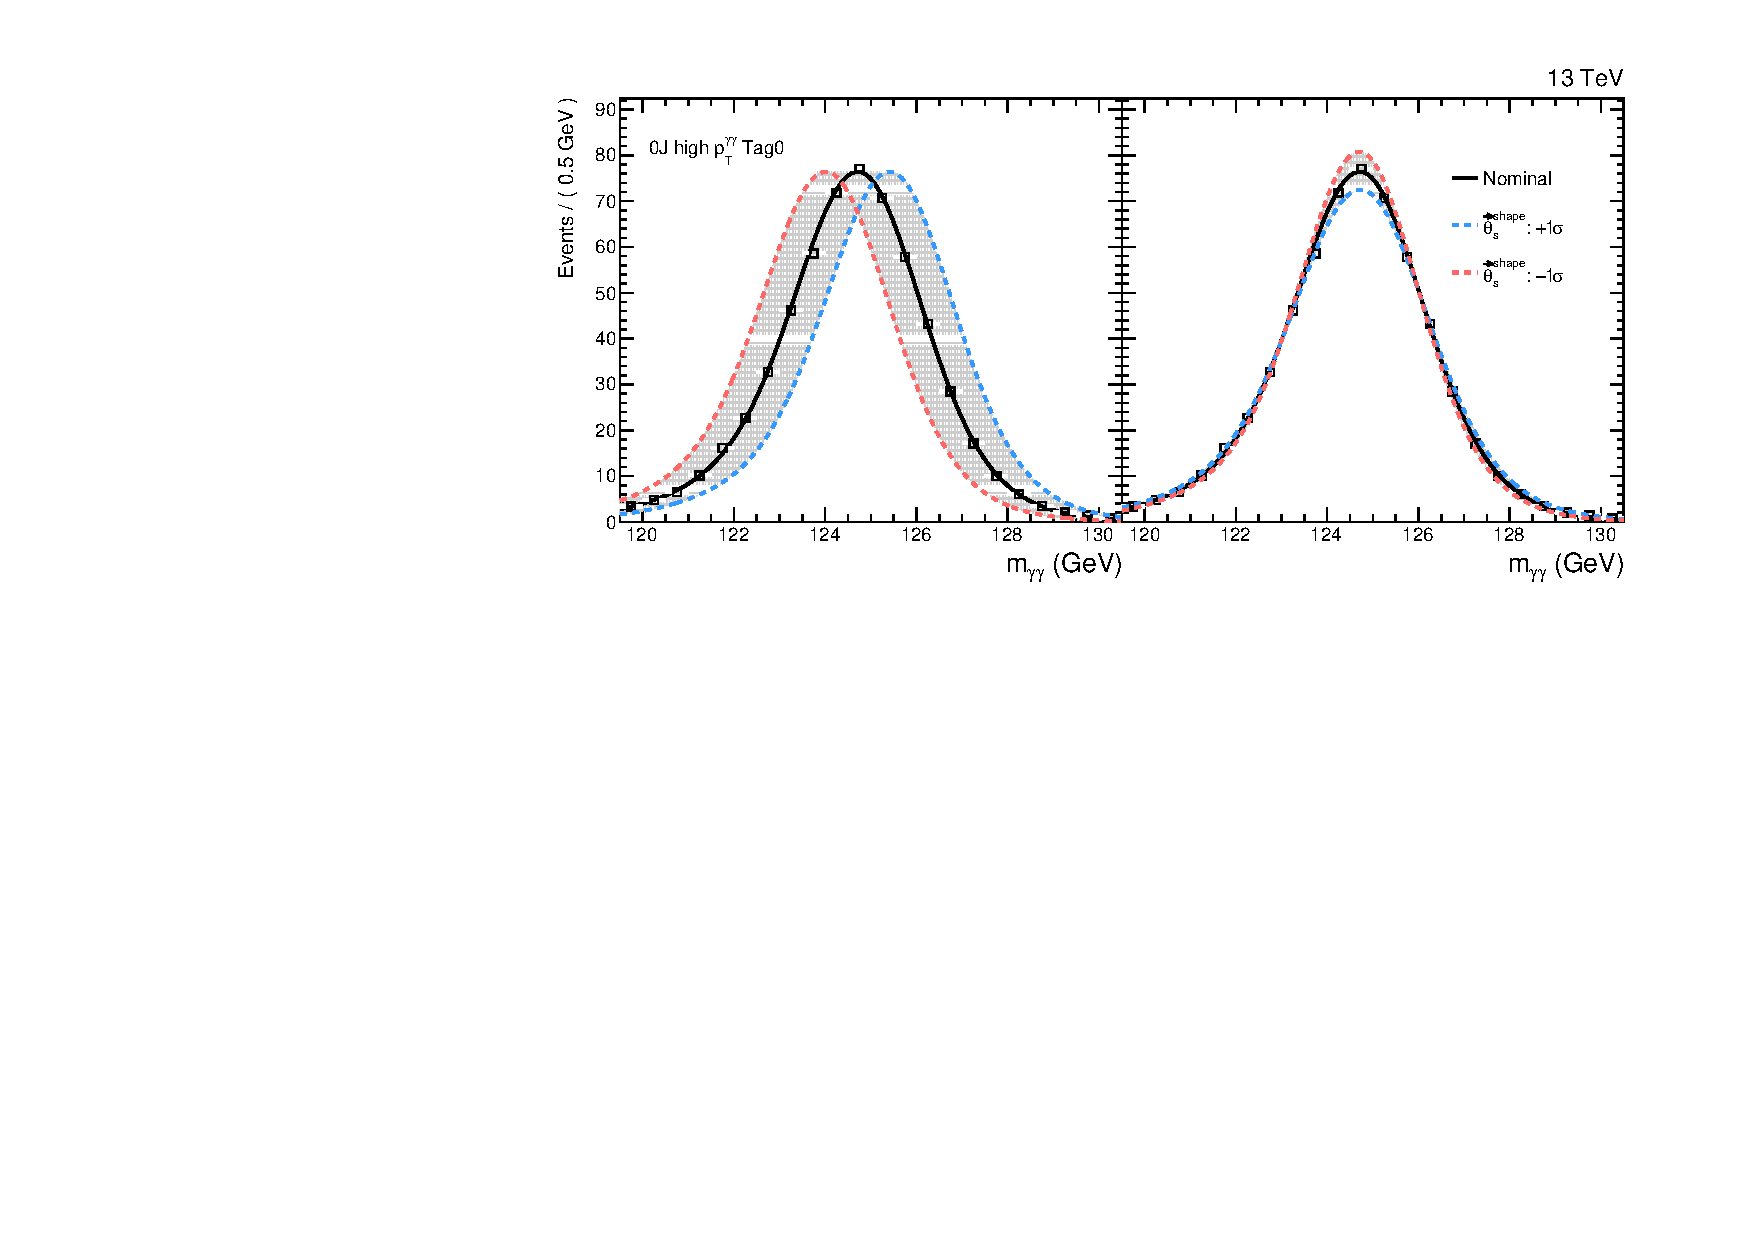
\includegraphics[width=1\textwidth]{Figures/hgg_stats/shapeSyst_withVertex_dropHighR9.pdf}
  \caption[Signal shape systematic uncertainties]
  {
    The impact of the signal shape uncertainties on the 0J high \ptgg Tag0 per-category model, decomposed into the maximum effect on the mean (left) and width (right). All nuisance parameters, $\vec{\theta}^{\,\rm{shape}}_{s}$, are shifted to plus 1$\sigma$ (blue dashed line) and minus 1$\sigma$ (red dashed line) of their nominal values. The maximum absolute variation in the mean is around 0.7~GeV, whilst the maximum relative variation in the width is approximately 5\%.
  }
  \label{fig:systematics_sigshape}
\end{figure}


\subsubsection{Yield uncertainties}
The experimental sources of uncertainty that only modify the event yield estimates are listed below. This includes the uncertainties in the luminosity, $\vec{\theta}^{\,\rm{lumi}}_{s}$, and those affecting the efficiency times acceptance of the event selection, $\vec{\theta}^{\,\epsilon,{\rm{exp}}}_{s}$. In general, the magnitude of the yield variation is calculated by varying the uncertainty source in simulation, propagating the events to the final analysis categories, and comparing the systematic-varied yield to the nominal. The combined effect of these uncertainties on the inclusive Higgs boson signal strength measurement is between 3 and 4\%.

\begin{itemize}
    \item \textit{Integrated luminosity}: uncertainties of 2.5\%, 2.3\%, and 2.5\% are determined by the CMS luminosity monitoring for the 2016, 2017, and 2018 data sets respectively~\cite{CMS-PAS-LUM-17-001,CMS-PAS-LUM-17-004,CMS-PAS-LUM-18-002}, whilst the uncertainty on the total integrated luminosity of all three years in 1.8\%. A partial correlation scheme is introduced to account for common sources of uncertainty in the luminosity measurements of each year. In total, this amounts to defining three uncorrelated and six correlated nuisance parameters.
    
    \item \textit{Photon preselection}: the photon preselection efficiency scale factors are derived using the tag-and-probe method on \Zee events. This amounts to estimating the number of probes passing and failing selection by fitting a signal plus background model to the dielectron invariant mass distribution. The largest source of uncertainty is from the choice of signal hypothesis, and is estimated by fitting an alternative signal shape. Propagating to the category yields, the impact is less than 1\%. An additional uncertainty is included for the electron-veto scale factor, calculated using \Zmumug events, which has an even smaller impact on the yield, typically less than 0.5\%. 
    
    \item \textit{Trigger efficiency}: again  the trigger efficiency scale factors are measured with \Zee events using the tag-and-probe technique, and the size of the uncertainty is also less than 1\%. An additional source is included to account for a gradual shift in the timing of the inputs of the ECAL L1 trigger in the region $|\eta|>2.0$, which caused a specific trigger inefficiency during the 2016 and 2017 data taking. Both photons and to a greater extent jets can be affected by this inefficiency. The resulting uncertainty is largest for the categories targeting VBF production, with a maximum impact on the yield of around 1.4\%.
    
    \item \textit{Photon identification BDT score}: as discussed in section \ref{sec:photon_reconstruction}, the largest uncertainty in the photon identification originates from the limited size of the training sample in the CQR method. The size of the uncertainty is estimated by splitting the training sample in half and re-calculating the shower shape and isolation corrections. Figure \ref{fig:photon_id_1} shows this uncertainty (red band) successfully covers the residual discrepancies between data and simulation. The effect on the yield is then calculated by propagating this source of uncertainty through the full event categorisation, resulting in a variation of around 3\% for the most sensitive categories. 

    \item \textit{Per-photon energy resolution estimate}: the per-photon energy resolution estimate is an output of the photon energy regression and is used as an input feature in the event classifiers. The uncertainty in the resolution is parametrised as a $\pm$5\% variation about the nominal value, chosen to sufficiently cover all differences between data and simulation in the per-photon energy resolution distribution. The maximum yield variation in an analysis category from this source is around 5\%, however for most categories the impact is below the per-cent level. 
    
    \item \textit{Jet energy scale and smearing corrections}: the jet energy scale is calculated using the \pt balance of jets with Z bosons and photons in \Zee, \Zmumu and $\gamma$~+~j events, as well as the \pt balance between jets in dijet and multijet events~\cite{Khachatryan:2016kdb}. This energy scale is then used to correct the jet energies in simulation and data as a function of jet $p_T$ and $|\eta|$. The sources of uncertainty in this calculation arise from the absolute value of the scale, the relative $|\eta|$-dependence of the scale, pile-up mitigation and the detector response to different jet flavours. Over the full jet phase space considered in this analysis, the final uncertainties in the jet energy scale are below 3\%. Similar to the luminosity uncertainties, a partial correlation scheme is introduced, with correlations ranging between 0 and 100\%, to account for common sources of uncertainty in the jet energy scale measurement. Propagating this to the event yields, the impact is largest in categories targeting VBF, VH hadronic and top-associated production, and can be as high as 22\%.
    
    \noindent
    A separate nuisance is introduced to account for the uncertainty in the jet energy resolution calculation. The impact on the event yields is in general smaller than the jet energy scale uncertainties, but can be as high as 8\% for the most affected categories.

    \item \textit{Pileup jet identification}: the uncertainty in the pileup jet classification score is determined by comparing the scores of jets in events with a Z boson plus one balanced jet, in data and simulation. The effect on event categories with jet requirements is of the order~1\%.
    
    \item \textit{Missing transverse momentum}: the \met is used as an input variable in a number of event classifiers. The uncertainty in the \met is derived by shifting the reconstructed \pt of the physics objects entering the \met calculation, within the momentum scale and resolution uncertainties appropriate to each type of reconstructed object, as described in Ref~\cite{CMS-PAS-JME-16-003}. Independent nuisance parameters are defined for the \pt shifting of jets, photons, and unclustered objects. The impact on the category yields is never larger than 5\%, even for analysis categories that explicitly use the \met in the respective classifier.
    
    \item \textit{Lepton isolation and identification}: for both electrons and muons, the uncertainties in the isolation and identification are computed by varying the ratio of the efficiency measured in data and simulation, within uncertainties, where the efficiencies are calculated using the tag-and-probe technique on \Zee and \Zmumu events. The variations in the yields are less than 0.7\% in the ttH leptonic and tHq leptonic categories, 0.6\% in the WH leptonic categories and 1\% in the ZH leptonic categories. 
    
    \item \textit{Jet b tagging}: uncertainties in the b tagging efficiency are evaluated by comparing b tag discrimiator output distributions in data and simulation. The uncertainties include a statistical component on the estimate of heavy and light flavour jets in data and simulation. For top-associated categories, which make use of the b tagging discriminant, the variations in the yields are around 3\%.
\end{itemize}

\subsection{Theoretical uncertainties}\label{sec:systematics_theoretical}
The effect of all theory uncertainties are modelled using log-normal variations in the signal yield estimates (see equation~\ref{eq:lognormal}). Introduced in section \ref{sec:category_likelihood}, theory uncertainties contribute to the likelihood in two ways. Firstly, there are the uncertainties in the SM predictions of the cross sections and the \hgg branching fraction, $\vec{\theta}^{\,\rm{th}}_{s}$. The cross section uncertainties include both the inclusive per-production mode effects and the uncertainties which migrate events across STXS bin boundaries. As a result of the signal parametrisation used for the cross section measurements, shown in equation \ref{eq:mu_stxs}, uncertainties of this first type cancel in the ratio with equation \ref{eq:signal_yield}, and therefore do not enter the final fit likelihood. Instead, they are attributed to the uncertainties in the SM predictions of the measured quantities, represented by the hatched grey boxes in Figures~\ref{fig:stage0_results}, \ref{fig:stage1p2_maximal_results} and \ref{fig:stage1p2_minimal_results}. Conversely, for all interpretations of cross section measurements e.g. signal strengths, coupling modifiers or EFT parameters, the $\vec{\theta}^{\,\rm{th}}_{s}$ nuisance parameters are folded into the measurement i.e. included in the likelihood.

Originating from our lack of understanding of the underlying theory when simulating events, the second type of uncertainty, $\vec{\theta}^{\,\epsilon,{\rm{th}}}_{s}$, affects the acceptance of the analysis categories. For each uncertainty source, the total effect on each STXS bin is integrated out, providing a nuisance parameter that models the migration of events from a given STXS bin between analysis categories. In other words, this models the within-bin shape effects. When calculating the impact of these nuisance parameters, it is imperative to include events that do not enter any analysis category to ensure that the migration of events in and out-of-acceptance is accurately modelled. In contrast to the first type, these uncertainties enter the cross section measurements as variations in the calculated $\epsilon^{i,\gamma\gamma}_{k}$ values.

The different sources of theoretical uncertainty and their application via $\vec{\theta}^{\,\rm{th}}_{s}$ and $\vec{\theta}^{\,\epsilon,{\rm{th}}}_{s}$ nuisance parameters are described below.

\begin{itemize}
    \item \textit{Renormalisation and factorisation scales}: the uncertainty arising from varying the renormalisation and factorisation scales from the nominal value used to calculate the SM predictions for the cross sections, and to simulate the kinematic properties of the events. These uncertainties account for missing higher order terms in perturbative calculations, and reduce in size as the order of the calculation is increased. The recommendations from Ref.~\cite{deFlorian:2016spz} are used, where the $\pm$1$\sigma$ variations are displayed for the different Higgs boson production modes in Table~\ref{tab:qcdscale_variation}. The effect on the ggH cross section depends on the number of jets in the event.
    
    \begin{table}[htb]
        \caption[QCD scale uncertainties in production mode cross sections]{The QCD scale uncertainties in the production mode cross sections, expressed as percentage variations.}
        \label{tab:qcdscale_variation}
        % \vspace{.5cm}
        \centering
        \footnotesize
        \setlength{\tabcolsep}{3pt}
        \renewcommand{\arraystretch}{2}
        \begin{tabular}{c|c|c|c|c|c|c|c|c|c|c}
            ggH 0J & ggH 1J & ggH $\geq$2J & VBF & WH & ZH & ggZH & ttH & tHq & tHW & bbH   \\ \hline
            $\pm$3.8\%  & $\pm$5.2\%  & $\pm$8.9\% & $\pm$0.4\% & $^{+0.5}_{-0.7}$\% & $^{+3.8}_{-3.1}$\%  & $^{+25.1}_{-18.9}$\% & $^{+5.8}_{-9.2}$\% & $^{+6.5}_{-14.9}$\% & $^{+4.9}_{-6.7}$\% & $^{+20.2}_{-23.9}$\% \\ 
        \end{tabular}
    \end{table}

    \noindent
    An additional uncertainty is included for ggH production originating from the resummation of divergent terms in the perturbative expansion. The magnitude of this uncertainty is 0.1\% for 0J events, 4.5\% for 1J events, and 8.9\% for events with at-least two jets.
    
    The within-bin shape variations in the event kinematic properties originating from uncertainties in the QCD scale are modelled by recalculating the fraction of events in each category, $\epsilon^{i,\gamma\gamma}_{k}$, when changing the renormalisation and factorisation scales by a factor of two in the same direction simultaneously. These uncertainties, of type $\vec{\theta}^{\,\epsilon,{\rm{th}}}_{s}$, are decorrelated for different production modes and different regions of the Higgs boson phase space, resulting in 22 independent nuisance parameters. The magnitude of these within-bin uncertainties accounting for migrations between analysis categories are in general around 1\%, but can be as large as 5\% for off-diagonal elements in Figure \ref{fig:purity_matrix}.
    
    \item \textit{Modelling of ggH STXS fractions}: additional sources of uncertainty of type $\vec{\theta}^{\,\rm{th}}_{s}$ are included to account for the migration of events \textit{across} STXS bin boundaries, which therefore affect the SM predictions of the cross sections in each bin. These migration uncertainties are defined such that the total cross section of the summed bins, either side of the boundary, remains constant. In other words, the combined impact of such across-bin migration uncertainties cancels in the sum.
    
    \noindent
    In total, fifteen of such nuisance parameters are defined for ggH. Nine account for the uncertainty in the modelling of the \ptH distribution: four for migrations across the $\ptH$~=~200, 300, 450, and 650~GeV boundaries, one for the migration of 0J events across the $\ptH$~=~10~GeV, and four nuisances for migrations across the $\ptH$~=~60 and 120~GeV, defined independently for 1J and $\geq$2J events. Two nuisance parameters are defined to reflect migrations across the \mjj boundaries at 350 and 700~GeV, and a further two to account for the variations in the poorly-modelled \ptHjj variable, covering migrations across the 25~GeV boundary for events in different \mjj bins. Finally, two nuisances are included to account for the migration between the zero, one and two or more jet bins. 
    
    \noindent
    An additional source is included to model the uncertainty of ggH in the boosted regime. The flat value of 15\% is taken directly from Ref.~\cite{Becker:2020rjp}, and affects all ggH STXS bins with $\ptH>200$~GeV. Figure \ref{fig:ggH_uncertainty_scheme} shows the full set of $\vec{\theta}^{\,\rm{th}}_{s}$ nuisance parameters considered for ggH, and their relative impact on each STXS bin. The total magnitude of these uncertainties ranges from 6.5\% for ggH 0J high \ptH, to around 40\% for bins in the VBF-like region.
    
    \item \textit{Modelling of qqH STXS fractions}: in a similar fashion, a set of nine nuisance parameters are included to account for migrations across bin boundaries in the qqH STXS scheme. Six are used to model the uncertainty in the \mjj distribution, explicitly covering the migrations at $\mjj~=~$60, 120, 350, 700, 1000 and 1500~GeV. A further three nuisances are introduced for the boundaries at $\ptH~=~200$~GeV and $\ptHjj~=~25$~GeV for high dijet-mass events, and the migration of 0J and 1J events into the $\geq$2J region. The variations in cross sections arising from these migration uncertainties are typically below 3\%.
    
    \item \textit{Modelling of VH leptonic STXS fractions}: mis-modelling of the \ptV spectrum is covered by migration uncertainties defined for the boundaries at 75, 150 and 250~GeV. An additional nuisance parameter is included for events with \ptV between 150 and 250~GeV, to cover migrations across the 0J to greater than 1J boundary. These nuisances are defined independently for the WH, ZH, and ggZH production modes, resulting in 12 independent nuisance parameters. The values are similar for WH and ZH, being consistently lower than 6\%, but can be as large as 90\% for ggZH~\cite{ATL-PHYS-PUB-2018-035}. 
    
    \item \textit{Modelling of ttH STXS fractions}: four nuisance parameters are introduced to account for variations in the \ptH spectrum, defined for the boundaries at $\ptH~=~$60, 120, 200, and 300~GeV. The magnitude of these migration uncertainties are typically around 5\%, but can be as large as 10\% for the ttH~$\ptH<60$ STXS bin.
    
    \item \textit{Parton density functions}: uncertainties are included to reflect the limited precision in the composition of the colliding protons. As introduced in section \ref{sec:mc}, the PDF's describe the probability of finding a parton in the proton with a certain momentum fraction, $x$. Therefore, uncertainties in the parton density functions affect the likelihood of colliding partons, and in turn the cross section calculations and the event kinematics. The overall normalisation effect for each Higgs boson production mode is taken from Ref.~\cite{deFlorian:2016spz}. The impact is largest for the top-associated production modes, ranging from 3\% for ttH production to 6\% for tHW production.
    
    \noindent
    To evaluate the impact on the event kinematics, the PDF4LHC\_100 prescription~\cite{Ball:2014uwa,Butterworth:2015oua,Dulat:2015mca,Harland-Lang:2014zoa} is followed using the MC2\textsc{hessian} procedure~\cite{Carrazza:2015aoa,Gao:2013bia}. The nuisance parameters are of type, $\vec{\theta}^{\,\epsilon,{\rm{th}}}_{s}$ i.e. the overall effect on each STXS bin is integrated out to leave nuisance parameters describing the migration of events between analysis categories. In total, 60 independent nuisance parameters are introduced, which account for relatively small ($<$1\%) migrations between analysis categories.
    
    \item \textit{Strong force coupling constant, $\alpha_s$}: the uncertainty in $\alpha_s$ is treated along with the PDF uncertainties in the PDF4LHC prescription. In the same way, an overall normalisation effect is included for each Higgs boson production mode, and an additional $\vec{\theta}^{\,\epsilon,{\rm{th}}}_{s}$ nuisance parameter is included to model the variation in the event kinematics from changing the $\alpha_s$ value. The normalisation uncertainty is largest for ggH production, with a value of 2.6\%, whilst the within-bin migration uncertainty is in general smaller.
    
    \item \textit{Underlying event}: dedicated simulation samples are produced, where the tune of the event generator is modified. This varies the structure of the underlying event beneath the hard scattering process. This source of uncertainty is treated as a variation in the STXS bin cross sections, derived by comparing the STXS bin fractions to the nominal values. In general, the magnitude is less than 5\% but can be as high as 30\% for bins with high $p_T$ and a high number of jets.
    
    \item \textit{Parton shower}: in a similar way to the underlying event uncertainty, dedicated samples are produced changing the parton shower tune. Again, treated as an uncertainty in the cross section predictions, the impact is typically below 10\% but increases with the event \pt and number of jets. In particular, the qqH STXS bin boundaries that are sensitive to the presence of a third jet ($\ptHjj~=~$25~GeV) are greatly affected by this source of uncertainty, with impacts as high as 40\%. This is because the third jet in the event always originates from the parton showering, and not the matrix element of the hard process.
    
    \item \textit{Modelling of ggH contamination in the top-associated categories}: the theoretical predictions for ggH are less reliable in the region of phase space where the Higgs boson is produced in association with a large number of jets. Three independent nuisance parameters are introduced with a combined effect of around 50\% on the ggH yield in the top-associated categories. Firstly, the uncertainty in the parton shower is modelled by comparing the difference in jet multiplicity between tt+jets events in data and \textsc{MG5\_aMC@NLO} simulation~\cite{Sirunyan:2018ucr}. A second source of uncertainty originates from the gluon splitting modelling, estimated by measuring the quantity $\sigma({\rm{ttbb}})/\sigma({\rm{ttjj}})$ in both data and simulation, and scaling the fraction of ggH events with real $b$ quark jets in simulation by their ratio~\cite{CMS-PAS-TOP-16-010}. The final source of uncertainty originates from the limited size of the simulated sample, providing a small number of ggH events which enter the top-associated categories. The combined impact of these uncertainties in the top-associated signal strength measurement is about 2\%.
    
    \item \textit{$H\rightarrow\gamma\gamma$ branching fraction}: the probability of the Higgs boson decaying to photons is only known to within an uncertainty of 2\%~\cite{deFlorian:2016spz}. This uncertainty affects the inclusive signal yield estimate and hence is of type $\vec{\theta}^{\,\rm{th}}_{s}$.
\end{itemize}

\begin{figure}[htb]
  \centering
  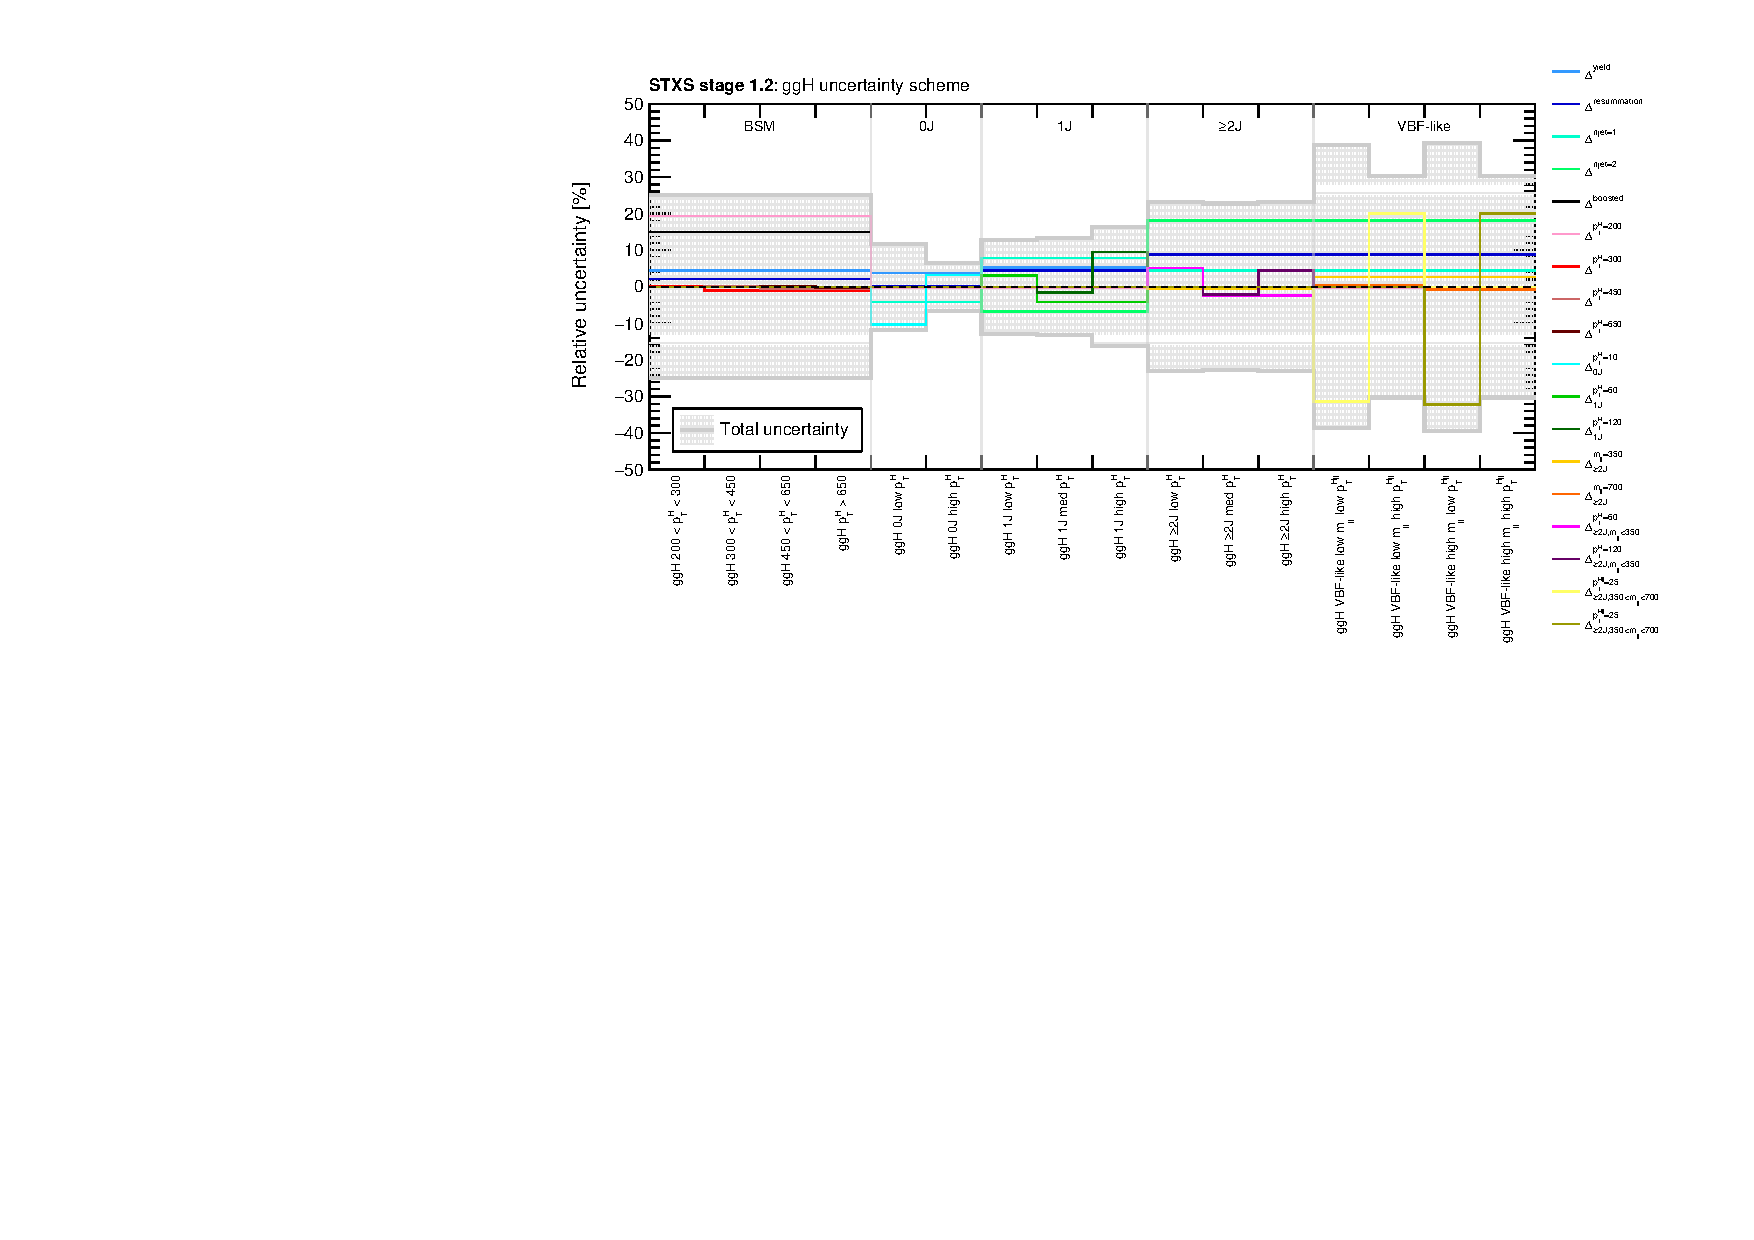
\includegraphics[width=1\textwidth]{Figures/hgg_stats/ggH_NPScheme.pdf}
  \caption[STXS stage 1.2 ggH uncertainty scheme]
  {
    The impact of the ggH theoretical uncertainties on each STXS stage 1.2 bin, expressed as a percentage variation in the nominal cross sections. The coloured lines show the impact from each individual nuisance parameter, whilst the filled histogram shows the total uncertainty, defined as the quadrature sum of all contributions.
  }
  \label{fig:ggH_uncertainty_scheme}
\end{figure}

As described later in section \ref{sec:results_STXS}, it is necessary to merge groups of STXS bins in the measurement to avoid large uncertainties or very high correlations between the measured cross sections. This induces an additional complication into the theory uncertainty scheme, such that the nuisance parameter representing the migration of events across the merged boundary must be introduced into the cross section measurement. Effectively, this act of merging re-defines the signal process and changes the across-bin migration uncertainty ($\vec{\theta}^{\,\rm{th}}_{s}$), to a within-merged-bin shape effect ($\vec{\theta}^{\,\epsilon,{\rm{th}}}_{s}$). For example, if the WH lep 0J $150<\ptV<250$, WH lep $\geq$1J $150<\ptV<250$ and WH lep $\ptV>250$ STXS bins are merged into a single parameter of interest, the nuisance parameters representing migrations across the $\ptV=250$~GeV boundary and the $N_{\rm{jets}}=1$ for $150<\ptV<250$~GeV boundary are included in the definition of the likelihood for the cross section measurement.

\section{Summary}
This chapter has introduced the method for the statistical inference of Higgs boson properties using high-energy proton-proton collision data, in particular for events consistent with the diphoton decay of the Higgs boson. Firstly, the construction of the per-category likelihood function and the subsequent method for extracting the results were described in detail. Following this, the various inputs to the likelihood function were covered. The signal model is constructed per year for each STXS bin in each analysis category, modelled as a sum of up to five Gaussian functions. The uncertainty in the choice of background functions is accounted for using the discrete profile likelihood method, where the exact form of the function in each analysis category is modelled using a discrete nuisance parameter. Systematic uncertainties regarding the signal estimate are incorporated as constrained nuisance parameters in the likelihood. Those which affect the signal shape are encoded directly as variations in the mean, width, and normalisation of the signal model Gaussian functions. The remaining experimental and theoretical uncertainties are modelled as log-normal variations in the yield estimates, calculated separately for each STXS stage bin in each analysis category.
